\documentclass[UTF8]{pkuthss}
\usepackage[backend = biber, style = caspervector, utf8, sorting = none]{biblatex}
\usepackage{multirow}
\usepackage{booktabs}
\usepackage {colortbl}
\setlength{\bibitemsep}{3bp}
\renewcommand*{\bibfont}{\zihao{5}\linespread{1.27}\selectfont}
\pkuthssinfo{
	cthesisname = {硕士研究生学位论文}, ethesisname = {Master Thesis},
	ctitle = {区块链加密货币的实时实名交易监督系统的设计与实现}, etitle = {Design and Implementation of Real-time Real-name Transaction Monitoring System Using Blockchain Cryptocurrency},
	cauthor = {陈伯韦},
	eauthor = {Chen Po Wei},
	studentid = {1601210903},
	date = {二〇一八 年 七 月 },
	school = {软件与微电子学院},
	cmajor = {软件工程专业}, emajor = {Data Mining and Business Intelligence},
	direction = {数据挖掘与商务智能方向},
	cmentor = {李杰 教授}, ementor = {Prof.\ Lijie},
	ckeywords = {比特币,区块链,多重签章}, ekeywords = {Bitcoin, Blockchain, Multiple signatures}
}
\addbibresource{thesis.bib}
\usepackage{color}
\def\pkuthssffaq{%
	\emph{\textcolor{red}{pkuthss 文档模版最常见问题:}}
	\texttt{\string\cite}、\texttt{\string\parencite} %
	和 \texttt{\string\supercite} 三个命令分别产生%
	未格式化的、带方括号的和上标且带方括号的引用标记:%
	\cite{test-en},\parencite{test-zh}、\supercite{test-en, test-zh}。

	若要避免章末空白页,请在调用 pkuthss 文档类时加入 \texttt{openany} 选项。

	如果编译时不出参考文献,
	请参考 \texttt{texdoc pkuthss}“问题及其解决”一章
	“其它可能存在的问题”一节中关于 biber 的说明。
}

\begin{document}
	% 以下为正文之前的部分,默认不进行章节编号。
	\frontmatter
	% 此后到下一 \pagestyle 命令之前不排版页眉或页脚。
	\pagestyle{empty}
	% 自动生成封面。
	\maketitle
	% 版权声明。封面要求单面打印,故需新开右页。
	\cleardoublepage
	\include{chap/copyright}

	% 此后到下一 \pagestyle 命令之前正常排版页眉和页脚。
	\cleardoublepage
	\pagestyle{plain}
	% 重置页码计数器,用大写罗马数字排版此部分页码。
	\setcounter{page}{0}
	\pagenumbering{Roman}
	% 中英文摘要。

	% Copyright (c) 2014,2016 Casper Ti. Vector
% Public domain.

\begin{cabstract}
	%\pkuthssffaq % 中文测试文字
	金融科技蓬勃發展的今天,區塊鏈技術也是重點發展對象。區塊鏈技術最著名的代表作,不外乎是於2009年中本聰提出的一篇名為比特幣:一種點對點式的電子現金系統》(Bitcoin: A Peer-to-Peer Electronic Cash System)論文\parencite{bitcoinpaper},奠定了區塊鏈技術的開始,以及於貨幣銀行學緊密的結合。比特幣是一個集成網路學、密碼學、金融學的密碼貨幣,現今的密碼貨幣市場中,有數以千計的貨幣種類在市場流動著。值得一提的是,於2009年開始運作至今(2018年),比特幣點對點式的電子現金系統,還未出現過錯誤,這也體現了比特幣可以承受將近十年來各式各樣的網路攻擊以及在程序上並無太大的漏洞瑕疵。比特幣最大的特色在於去中心化、匿名化,因為去中心化的基礎建構出一個政府無法管控的點對點的金流,也因為匿名,使得政府相關人士難以追查每一筆資金的真正持有者是誰,在傳統的中心化銀行跨國轉帳中都需要基本的實名制驗證,藉由實名制有效過濾洗錢的發生。但在比特幣點對點的電子現金系統中,沒有任何一個使用者或是政府可以要求每一個人的實名制,促使的交易追蹤、洗錢防制變得更加的困難。除了不可管控、難以追蹤的特點外,在國家政府方面稅收更是國家繼續運作的基礎資金來源,因為現今的國家並無支持比特幣相關的收銀機或是制定出相關的標準稅務,也使得國家政府無法在這方面獲得稅務資金。

	經由深度的了解比特幣的運作原理,再由上述無法管理資金流、無法追蹤、無法得到稅收,三項出發點,本論文致力於設計一個比特幣的收銀監督系統。在設計該系統前,也探討了多種場景下的交易模型,發現現金已經存在匿名支付給匿名、匿名支付給實名的模型,在刷卡支付中有著實名支付給實名、實名支付給匿名再支付給實名,上述的四種模型。經由上述的分析,可以得知,個人隱私的意識崛起,唯有匿名支付給實名時,才可以做到不透露消費者信息,亦可做到消費者權益的申訴權。在點對點的電子現金的市場中,還是停留在匿名支付給匿名的場景中,本論文致力於設計一個匿名支付實名的密碼貨幣市場的監督收銀系統,以實踐消費者匿名,同時也讓消費者擁有費者權益的交易模型。
\end{cabstract}

\begin{eabstract}
	Test of the English abstract.
\end{eabstract}

% vim:ts=4:sw=4

	% 自动生成目录。
	\setcounter{tocdepth}{1}
	\tableofcontents

	\renewcommand\listfigurename{图目录}
	\newcommand{\loflabel}{图}
	\renewcommand{\numberline}[1]{\loflabel~#1\hspace*{1em}}
	\listoffigures
	\renewcommand\listtablename{表目录}
	\newcommand{\lotlabel}{表}
	\renewcommand{\numberline}[1]{\lotlabel~#1\hspace*{1em}}
	\listoftables

	%% 以下为正文部分,默认要进行章节编号。
	\mainmatter
	% 序言。
	%% Copyright (c) 2014,2016 Casper Ti. Vector
% Public domain.
\specialchap{序言}


	% 各章节。
	% Copyright (c) 2014,2016 Casper Ti. Vect
 
\chapter{绪论}

	现金法定货币,交易凭据及交易数据库存在着一些缺点。如现金很难杜绝假钞的横行,交易凭据有着伪造的可能,在交易数据库中信息不一致,数据库被DDOS攻击,交易数据被窜改,数据库损毁,都是在传统交易过程中曾出现过的窘境。

	于2009年加密货币 - 比特币\supercite{bitcoinpaper}的问世,以密码学、网络学与货币银行学为基础创建了新一代的网络货币。各式网络货币中又以比特币最为广泛使用,其防堵被窜改、公开交易数据查看、使⽤者具匿名性、⾃动运作不须⼈为运营等等多项特性深受现今用户喜爱。至今区块链技术已成为IBM、摩根大通、微软、谷歌与英特尔等重点开发项目,被视为改善银行运作效率、降低运营成本、提升信息安全、创建公开数据的最佳方法。为解决现金、收益及交易数据库存在之问题,本文采用以区块链为基础的加密货币比特币为基础,进行商业化收银系统开发。不仅是基于⽐特币算法稳定、交易公开透明、不可被窜改等特性,同时本论⽂更加⼊监督标签,促使在匿名交易转为部分实名交易之过程中,监管部⾨能有更好的新兴货币技术的提升,亦可创建自动化的税务审查机制,大幅降低人事成本,进而实现提升交易系统信息之可靠度与其稳定性。

	\section{选题背景}

		追溯着加密货币市场的演进,于2009年时,比特币并非第一个加密货币,在比特币之前已经有着很多类似的加密货币开发实验,但是一直无法做出一个稳定点对点式的电子现金系统,关于其制作瓶颈之部分将于后段章节阐述。在比特币稳定发展之后,有着许多对比特币有兴趣的研究者,以稳定的比特币系统为基础修改了许多基本的协议。于2011年相继创造出了货币,将其称之为⼭寨币。山寨币早期较为著名包括有莱特币(Litecoin,LTC)\supercite{litecoin}、狗币(Dogecoin,DOGE)\supercite{dogecoin}、域名币(Namecoin,NMC)\supercite{namecoin},于2014年也有人认为比特币挖矿使用到了大量的哈希运算,这样的大量运算也浪费了许多的社会资源,进而开发出较具意义的工作量证明挖矿算法,其中较为著名的如素数币(Primecoin,XPM)\supercite{primecoin}。 于2015年底也诞生了现在最为著名的以太坊经典(Ethereum Classic,ETC)\supercite{ethereumclassic}、以太坊(Ethereum,ETH)\supercite{ethereum},以太坊最重⼤突破设计在于将编程语⾔虚拟机移植到了区块链架构上,这使得区块链技术不再仅止于点对点的电⼦现⾦系统,也创造出了属于以太坊的编程语言Solidity\supercite{solidity},使以太坊在虚拟机(Ethereum Virtual Machine,EVM)\supercite{Ethereum:Asecuredecentralisedgeneralisedtransactionledger}中可以使⽤Solidity 创建智能合约,合约可以建构去中心化的应用程序,如去中心化的交易所,将交易所去中心化可以有效的防治DDOS攻击 \supercite{Bitcoin:Economicstechnologyandgovernance},降低交易所因为黑客攻击而倒闭的可能性。
		

		\subsection{加密货币市场}

		加密货币中最具代表性的是比特币,但除了比特币之外也存在许多模仿比特币的加密货币,有的是为其利益,有的是鉴于比特币的各种不足,进而希望借由其他货币改善⽐特币不够完美之处。加密货币市场中有成千上万种的加密货币,其中较广为人知的加密货币会在Cryptocurrency Market Capitalizations\supercite{CryptocurrencyMarketCapitalizations}的排行榜中出现,截至2018年2月8日该排行榜已经收入了1510种加密货币。在Cryptocurrency Market Capitalizations统计的数据当中,可知整体的加密货币市场,如图\ref{TotalMarketCapitalization}所示,于2018年1月7日创下了历史新高,加密货币市场的总市值也高达了829,579,000,000美金,相当于五兆人民币的总市值。

		\begin{figure}[!htbp]
			\centering
			\includegraphics[width = 1\textwidth]{TotalMarketCapitalization.png}
			\caption{2017年1月21日到2018年1月21日期间加密货币总市值走势图\supercite{CryptocurrencyMarketCapitalizations}}\label{TotalMarketCapitalization}
		\end{figure}

		经由Cryptocurrency Market Capitalizations数据显示,整体加密货币市场自2013年起已经高达150亿美金,2014年与2015年间总市值减少到近乎2013年的一半。针对比特币的价格波动,论文"Have the security flaws surrounding Bitcoin effected the currency's value?."
		\supercite{HavethesecurityflawssurroundingBITCOINeffectedthecurrencysvalue?}
		作出详尽的市场调研,致力于探讨在各个比特币市场大事件中对比特币价格的波动影响,针对影响的程度该论文给出影响指数,当中影响最为严重的是于2014年2月发生的日本交易所Mt.Gox倒闭事件,因为早期的加密货币市场中无完善的法律规范,各国对加密货币的接受度有所不同,日本对金融科技的接受度相较于较为开放的情况下成立了全世界第一家比特币交易所Mt.Gox,也因为交易所不够普及,使得大部分的加密货币交易都集中在Mt.Gox交易所中,使Mt.Gox 倒闭事件成为震荡市场价格重⼤因⼦之⼀,也造成2014与2015年的加密货币市场低迷。而在2017年,比特币又以2016年总市值之35倍的姿态攀上新高点,主要是因为美国最大的期权交易中心芝加哥期权交易所(Chicago Board Options Exchange, CBOE)于2017年12月10日宣布支持比特币期货交易,此举将比特币价格推升到20,000美金的历史新高,图\ref{Thetotalmarketcapitalization}为2013年至2018年间比特币总市值K线图。

			\begin{figure}[!htbp]
				\centering
				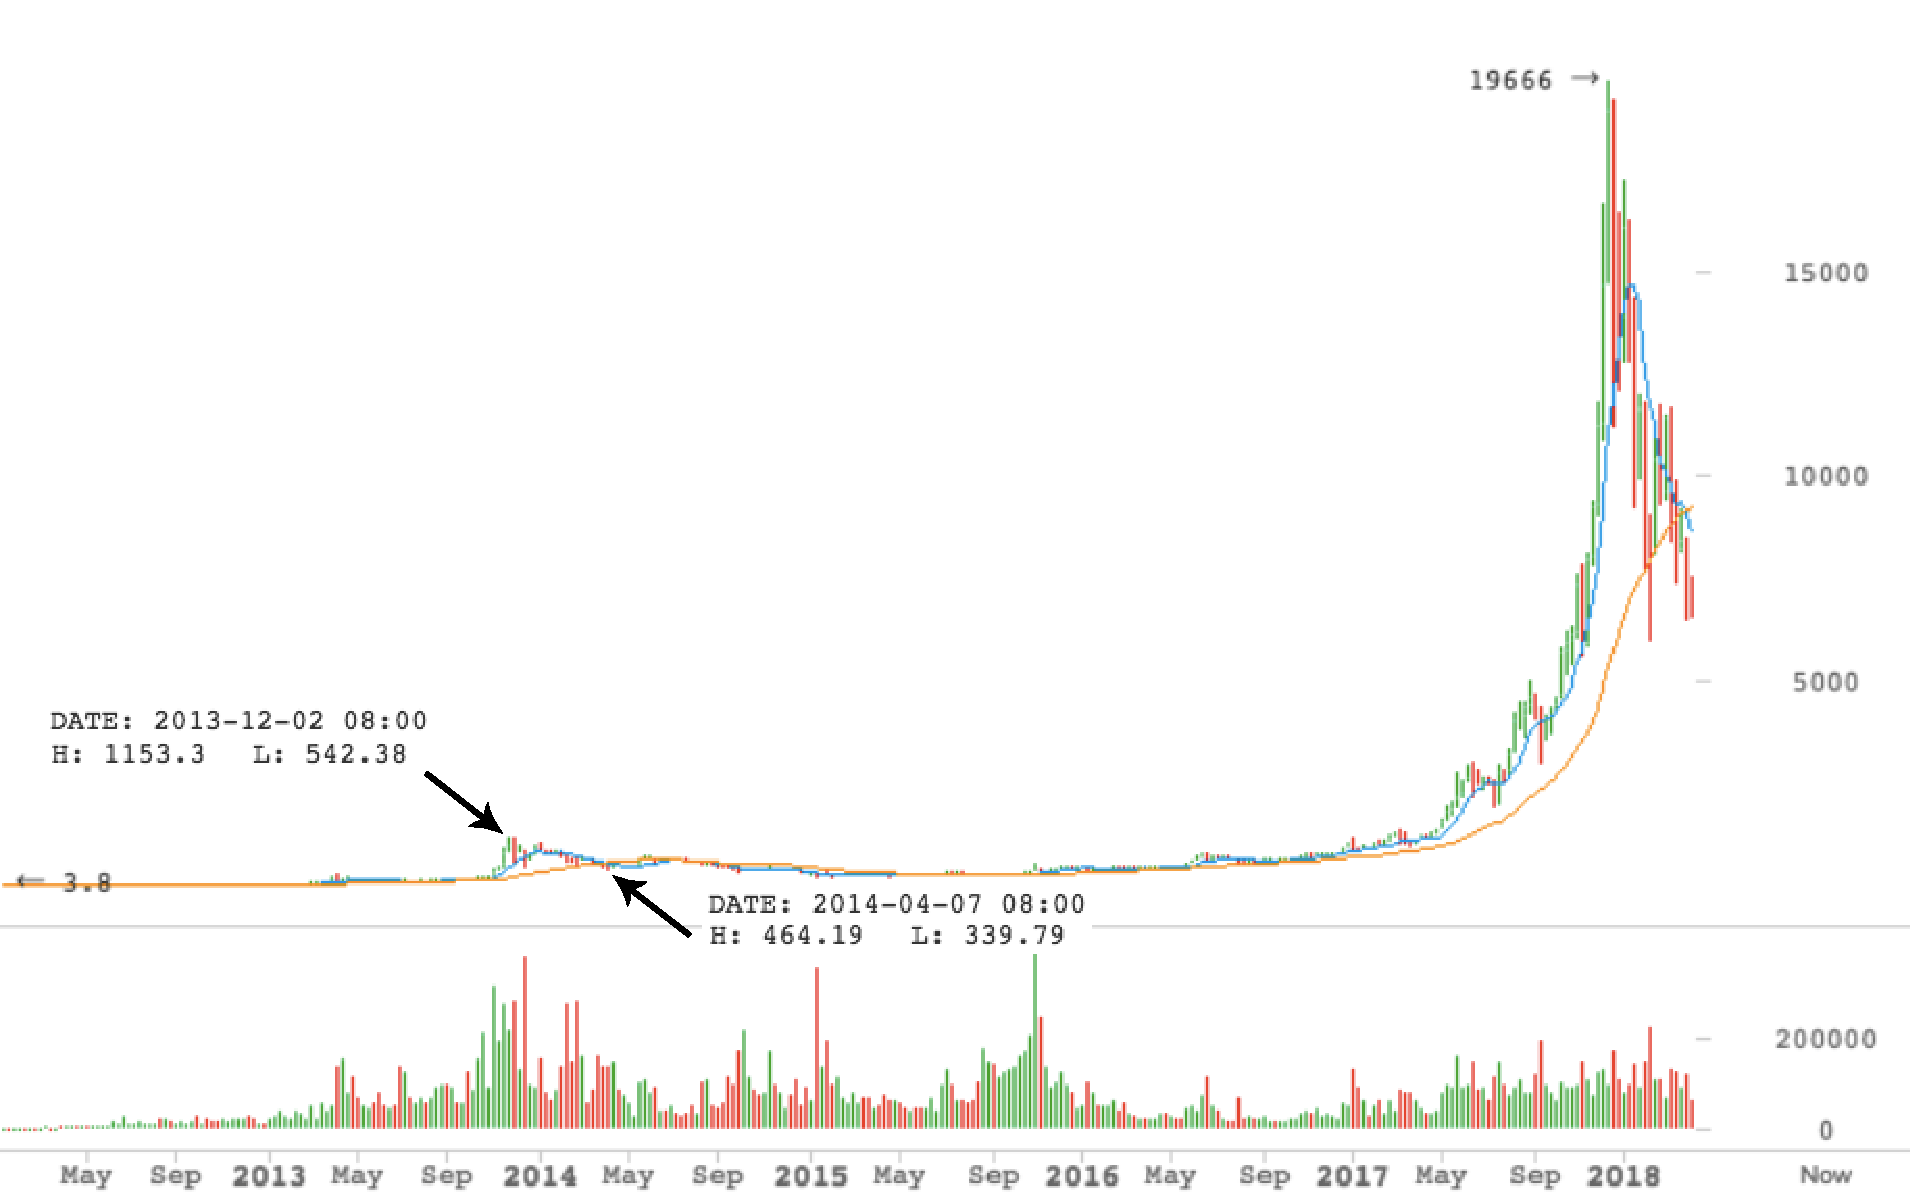
\includegraphics[width = 1\textwidth]{Thetotalmarketcapitalization.jpg}
				\caption{2013年至2018年间比特币总市值K线图\supercite{CryptocurrencyMarketCapitalizations}}\label{Thetotalmarketcapitalization}
			\end{figure}
		

			\subsection{加密货币的优势}
			于2009年Satoshi Nakamoto发布了比特币系统,成为全世界第一个加密货币的雏形。其透明的交易信息、区块链交易数据无法修改和删除、匿名与⾃治系统等特性,促使区块链技术冲破现存传统中⼼化之⾦融机构技术上的籓篱。以下将逐一说明加密货币的七项优点,分别为区块链结算系统不间断的运行、远距离支付、货币为用户持有、开放和透明的交易信息、区块链交易数据无法修改和删除、交易匿名性以及自治性系统。

				第一,区块链结算系统不间断的运行。基于区块链技术与点对点网络的架构,以比特币为例,自2009年至今,所有的比特币交易事件皆会存储在比特币区块链当中,区块链既无法删除也无法修改,比特币区块链会以点对点网络的方式存储在比特币网络中的全节点\supercite{YouReallyShouldRunaBitcoinFullNode:HeresWhy},目前比特币网络中的全节点高达11147个。与传统中心化的银行数据库相比,可能会因为银行的服务器维护,导致交易无法顺利进行,甚至可能有黑客的入侵导致银行或是个人资产有重大的损失。点对点网络提供稳定的数据库元数据,不会因为数据库的停机而无法继续使用,实现其24小时不间断之运作。
				
				第二,基于点对点网络架构完成远距离支付。于跨国汇款从美国转帐至中国一百万美金的场景中,需要经过的手续较为繁琐,资金有可能需要经过多个国家才可以抵达目的地,在经过各个国家的过程中,需要支付各国的手续费,也需要等待各个国家办理该业务的时间,即使当资金顺利抵达了目的地银行,目的地银行也需要花将近三至五日的工作日确认该笔金额的来源。届时领款人亦需要前往银行核实完整的身份验证、解释资金用途,才得以领取这笔跨国资金。比特币系统当中,有着24小时不间断运作的优点,也因为点对点网络架构,使得比特币无需经由传统金融机构繁琐的步骤完成国际汇款,于比特币系统中无系统壅塞的情况下,平均10分钟即可入帐,实现其短时间内即可完成远距离支付之运作。

				第三,加密货币为用户持有。传统的金融体系中,资金的存储、流动往往需要经过银行,用户将所有的资产存入银行,拿到的是一串数字的银行余额,银行是一个中心化的机构,有着最高的权利。中央社的新闻\supercite{Bankguardsstolen}指出,台湾各地于2017年接连于土地银行、日盛银行、彰化银行、京城银行、兆丰银行皆传出银行行员监守自盗的行为,总金额高达一亿三千万新台币。在比特币系统中,比特币有如金币般存放在个人的比特币地址当中,用户为真实持有着货币,即使是比特币系统亦无权利动用该笔比特币资产,唯有比特币地址的私钥持有者,才可以转移该笔比特币地址中的比特币资产。

				第四,公开的交易信息。基于区块链架构,所有的交易信息皆以公开的方式存储于区块链中,并且可信任与方便的取得元数据,以下将针对可信任与元数据进行探讨。
				\begin{enumerate}
					\item 可信任:在公有链的基本架构上,所有的交易记录都是公开透明的存储在区块链当中,比特币网络的用户都可以查看该笔交易,所有人都可以检查每个交易记录的正确性,公开的交易信息亦提升交易数据之可信性。
					\item 元数据:除了以区块链技术为基础建构出可信任的系统之外,开放和透明的特性让更多的开发商或新公司得以更容易获得交易的元数据。毕竟,在传统金融体系中,所有交易记录均由中央金融机构存储,从中央金融机构提取原始交易信息并不容易,区块链的开放性和透明性促使金融公司降低了获取原始数据努力的门槛。公司或学者可以透过元数据制定出可视化的开发计划,甚至可以运用大量数据来分析前所未达的新价值观点。
				\end{enumerate}

				第五,区块链交易数据无法修改和删除。在区块链结构中,通过严格验证的所有信息都记录在区块链中,且用户及系统平台都不赋与删除及修改之权限。根据区块链的特点,旧区块的哈希值在连接区块链的过程中,旧区块的哈希值会被存储在新区块。只要区块中的值被修改,即使仅有1 bit的变化,也会产出完全不同的哈希值,这也就是所谓的雪崩效应(Avalanche effect)\supercite{Theuseofbentsequencestoachievehigher-orderstrictavalanchecriterioninS-boxdesign}。由于上述结构特性,区块链中所有的信息都会被系统纪录且都不会被改变,倘若区块中记载的比特币交易在其中一个比特币全节点验证的结果被窜改,则该区块将不被比特币系统接受。因此,所有已经存储在区块链中的交易记录将不能被修改和删除,进而实现其架构安全之稳固。

				第六,区块链系统中所有的用户皆为匿名。现今社会中,个人信息保护已成为企业最重要的课题。在区块链系统中创建的所有帐户都不会与真实世界中的实体创建直接关联,也因为没直接关联所以创建匿名。区块链系统中的所有帐户都是由匿名个体创建,匿名的设计可以有效保护消费者的隐私。然而,VISA交易与比特币系统截然不同,在使用VISA支付系统前,用户必须向VISA公司的主机提交大量个人信息,这可能会产生个人信息泄露的风险。在区块链技术中,其匿名之特性可以有效地避免这个问题。

				第七,自治系统。在区块链系统中,区块链的运作依赖于一些算法,包括共识算法。因此,在这种自治系统中,没有人(例如节点或矿工)可以直接改变系统运作的规则。如果在比特币系统中发现需要更正的严重错误,可以使用比特币改进提案(Bitcoin Improvement Proposals,BIP)\supercite{BitcoinImprovementProposals}升级比特币系统。 在实施比特币改进提案之前,提议的比特币改进提案需要得到比特币系统中超过一定数量的矿工算力支持。由于这种以投票机制升级系统的门槛相当高,使得区块链系统通常不会有大的变化,因为变化不⼤也突显其相对稳定性。

			\subsection{加密货币的劣势}
			在区块链技术中,有着三项瓶颈,分别为每秒处理的交易量(Transactions Per Second,TPS)仅为7笔的限制、洗钱防治困难、低可扩展性,以下将逐一探讨。

				第一,每秒处理的交易量上限仅为7笔。图\ref{TPS}为国际上较为广泛使用的⽀付系统之每秒⽀持交易量⽐较图,以VISA为例,其以公司中心化运营的方式可以支持高达每秒2,000笔交易。但是以区块链技术为基础的比特币最大能够接受的每秒处理交易量仅为7笔。一般认为只要提升区块大小的限制,就可以提升每秒处理的交易量。提升每秒处理交易量的同时将产生下述的两项问题,分别为区块链成长速度过快造成节点崩溃以及区块同步延迟造成区块链分岔:

					\begin{figure}[!htbp]
						\centering
						\includegraphics[width = .6\textwidth]{TPS.png}
						\caption{Bitcoin、Western Union\supercite{WesternUnion}、PayPal\supercite{PayPal}以及VISA每秒支持交易量比较图\supercite{digibyte}}\label{TPS}
					\end{figure}

					\begin{figure}[!htbp]
						\centering
						\includegraphics[width = .8\textwidth]{blockchainsize.png}
						\caption{比特币区块链成长走势图\supercite{blockchainsize}}\label{blockchainsize}
					\end{figure}


					\begin{enumerate}
						\item 区块链成⾧速度过快造成节点崩溃。区块链成长速度过快会造成比特币全节点不堪负荷:从2009年至今的比特币区块链大小已达到188.89 GB,这样的成长速度因为比特币区块大小的最大值被设置为1 MB。图\ref{blockchainsize}为过去比特区块链大小,图中可以发现,于2016年开始,比特币区块链的成长速度为一直线,这表示着比特币网络中持续维持在供不应求的状况。为解决比特币每秒⽀持交易量上限的窘迫,现今对⽐特币的每秒处理交易量有许多优化的⽅案,其中包括解除比特币区块大小1 MB的限制。在一个区块上限为1 MB的限制下,满载的比特币系统中,比特币区块链平均每十分钟会增1 MB,每小时会增加6 MB,每天会增加144 MB,每月会增加4.2 GB,每年会增加高达50 GB,要达到1 TB的区块链大小还需要8年,在8年后的未来存储1 TB的数据量应该不会有太大的负担。倘若解除1 MB的区块限制,在系统的每秒处理交易量看似可以接受更多的交易成倍成长,面临1 TB的比特币区块链数据会在更短的时间内出现,倘若存储区块链的成本超过了摩尔定律的成长曲线,会进一步造成用户自愿成为比特币全节点的意愿度降低,使得比特币网络的全节点数变少,导致比特币点对点网络逐渐转向中心化网络发展,失去一开始点对点网络的意义。

						\item 造成区块链最新区块同步延迟而使区块链分岔。对于区块链的区块同步延迟同时也会造成比特币网络的影响,J. Göbel于"Increased block size and Bitcoin blockchain dynamics"\supercite{TelecommunicationNetworksandApplicationsConferenceITNAC201727thInternational}有着详细的研究,在上修区块大小上限的议题上,用户因系统占用量提高,⾃愿成为⽐特币全节点意愿度下降,此举可能对⽐特币点对点网络建构出的区块链同步上造成延迟,在11147个比特币全节点当中,平均每十分钟会有矿工于其中一个全节点生成一个最新的区块,该最新的区块会以点对点网络协议同步到其他11146个节点上。在比特币系统中,长年来的过程经验可以发现在矿工生成1MB的区块后同步到全网节点可以在创造下一个区块之前完成。倘若将区块大小修改为2MB或是更大,会使得比特币全节点的最新区块同步延迟现象更加明显,同步延迟会使得区块链分岔,造成11147个比特币全节点的信息不一致,近一步造成整个比特币点对点网络崩溃。
					\end{enumerate}
					

				第二,洗钱防治困难。匿名性为比特币系统一大特色,比特币的地址生成的熵是256 bits,乱数是在$2^{256}$的组态空间中随机选取,这样的地址与现实生活中的身份并无任何关联,使得黑市交易、洗钱防治变的困难,甚至有更为前沿的加密货币Monero\supercite{noether2014monero}导入了环签章(Ring Signature)\supercite{Thresholdringsignaturesandapplicationstoad-hocgroups}算法、Zcash\supercite{zhong2002faster}导入零知识证明算法\supercite{Zero-KnowledgeProofsofIdentity},使得原本公开透明的区块链,变得无法查看,进而造成加密货币在洗钱防治上更加的困难。2017年由Thibault de Balthasar and Julio Hernandez-Castro 所提出的论文"An Analysis of Bitcoin Laundry Services."\supercite{AnAnalysisofBitcoinLaundryServices},致⼒探究⽐特币匿名交易下的资⾦流动模型,试图以机械学习的方法找出比特币洗钱模型作为洗钱的工具,图\ref{Darklaunderworkflow}为该论文针对黑市交易中的洗钱服务运营商Darklaunder进行洗钱机
					\begin{figure}[!htbp]
						\centering
						\includegraphics[width = .6\textwidth]{Darklaunderworkflow.png}
						\caption{Darklaunder 洗钱模型\supercite{AnAnalysisofBitcoinLaundryServices}}\label{Darklaunderworkflow}
					\end{figure}

				第三,低可扩展性。区块链架构为了防止各式的攻击,所以在架构订定以及接口设计都有着严谨的规范。以下将阐述造成比特币低可扩展性的原因:

					\begin{enumerate}

						\item 修改比特币协议制作添加外部信息的区块链:比特币区块链技术是一个严谨的架构,倘若要创造可以支持外部信息的结构需要重新创造全新的加密货币,大部分的加密货币不支持外部输入,由于外部的信息输⼊无法保证其信息的正确性,近一步造成垃圾进垃圾出(Garbage In, Garbage Out,GIGO)的问题,倘若错误的信息存储在无法删除、修改的区块链下,只是强化该笔错误信息的错误。如食品履历区块链,致力于将食品生产到超市的过程逐一记录在区块链上,但如果一开始在输入信息时,无法保证其信息之正确性,则该食品履历区块链则毫无意义,错误的信息内容甚至可能使该错误被强化。

						\item 于区块头或交易信息添加外部信息:比特币区块链上,可以添加一些信息于区块上,该信息会永久保存于区块链上,除了在区块上添加信息,在比特币单笔交易信息上,亦可填写一些私人信息,但这样的空间大小有限,且现今的比特币价格日趋上涨,比特币交易手续费是以单笔交易大小计算,这将使得在交易中添加些个人信息变得更加昂贵。

					\end{enumerate}

				在比特币系统中,其区块链仅用于记录交易记录,不能扩展更多功能和应用程序。有很多开发者希望将比特币系统扩展到智能合约等其他应用程序。但是,后来发现改变原始比特币系统框架是具有挑战性的工作。因此,全球第二大加密货币以太坊(Ethereum,ETH)的作者Vitalik选择了创建了以太坊虚拟机(Ethereum Virtual Machine,EVM),而非改变原始的比特币系统框架。以太坊虚拟机所创建的智能合约可以在统一的以太坊平台上运行,而以太坊也借此突破了比特币之技术瓶颈。
	
	\subsection{国际情势分析}
	\begin{table}[!htbp]
		\centering
		\caption{各国政府对比特币态度统整表}
		\label{world}
		\begin{tabular}{@{}|l|l|c|c|l|@{}}
		\toprule
		\multicolumn{1}{|c|}{\multirow{2}{*}{序号}} & \multicolumn{1}{c|}{\multirow{2}{*}{国家}} & \multicolumn{2}{c|}{接纳} & \multicolumn{1}{c|}{\multirow{2}{*}{禁止}} \\ \cmidrule(lr){3-4}
		\multicolumn{1}{|c|}{} & \multicolumn{1}{c|}{} & 欢迎/放任 & 监管 & \multicolumn{1}{c|}{} \\ \midrule
		1 & 伊朗 & \begin{tabular}[c]{@{}c@{}}监管得当欢迎\\ 比特币发展\end{tabular} &  &  \\ \midrule
		2 & 以色列 & \begin{tabular}[c]{@{}c@{}}欢迎:欲发展\\ 国际ICO中心\end{tabular} &  &  \\ \midrule
		3 & 法国 & \begin{tabular}[c]{@{}c@{}}放任:与实体\\ 经济无关\end{tabular} &  &  \\ \midrule
		4 & 美国 & 暂不构成威胁 &  &  \\ \midrule
		5 & 新加坡 & \begin{tabular}[c]{@{}c@{}}不监管但注意\\ 周边活动\end{tabular} &  &  \\ \midrule
		6 & \begin{tabular}[c]{@{}l@{}}沙特阿拉\\ 伯王国\end{tabular} & \begin{tabular}[c]{@{}c@{}}加密货币尚未\\ 成熟,不监管\end{tabular} &  &  \\ \midrule
		7 & 乌克兰 & 不属于货币 &  &  \\ \midrule
		8 & 韩国 &  & \begin{tabular}[c]{@{}c@{}}很快将监管\\ 交易所\end{tabular} &  \\ \midrule
		9 & 菲律宾 &  & 计划监管ICO &  \\ \midrule
		10 & 英国 &  & 考虑监管 &  \\ \midrule
		11 & 马来西亚 & \multicolumn{1}{l|}{} & 范式监管框架 & \multicolumn{1}{c|}{} \\ \midrule
		12 & 俄罗斯 & \multicolumn{1}{l|}{} & \begin{tabular}[c]{@{}c@{}}2018年7月前\\ 完成立法\end{tabular} & \multicolumn{1}{c|}{} \\ \midrule
		13 & 日本 & \multicolumn{1}{l|}{} & \begin{tabular}[c]{@{}c@{}}任命加密货币\\ 监察长\end{tabular} & \multicolumn{1}{c|}{} \\ \midrule
		14 & 香港 & \multicolumn{1}{l|}{} & ICO须受法规监管 & \multicolumn{1}{c|}{} \\ \midrule
		15 & 津巴布韦 & \multicolumn{1}{l|}{} &  & \multicolumn{1}{c|}{定法前,属非法} \\ \midrule
		16 & 摩洛哥 & \multicolumn{1}{l|}{} &  & \multicolumn{1}{c|}{禁止加密货币交易} \\ \midrule
		17 & 印尼 & \multicolumn{1}{l|}{} &  & \multicolumn{1}{c|}{\begin{tabular}[c]{@{}c@{}}2018年前\\ 全面禁止\end{tabular}} \\ \midrule
		18 & 中国 & \multicolumn{1}{l|}{} &  & \multicolumn{1}{c|}{禁止加密货币} \\ \bottomrule
		\end{tabular}
		\end{table}
	
	比特币是一种全新的价值交换的媒介,因为区块链技术相当新颖,在各个国家所秉持的态度皆有所不同,大致可将各个国家对比特币的政策分为两大类,分别为接纳与禁止;在接纳加密货币的分类当中又分为欢迎、放任以及监管。

	在欢迎、放任的政策下的国家包括伊朗、以色列、法国、美国、沙特阿拉伯王国、乌克兰以及新加坡,上述国家政策上皆已抱持着开放且不监管的方式接纳加密货币,这些国家认为加密货币对于国家金融科技的发展具有前景;在分类于接纳但是实施监管的国家中,包括韩国、菲律宾、英国、马来西亚、俄罗斯、日本以及香港地区皆认为加密货币技术可能存在的高风险,且针对加密货币的洗钱防制以及非法集资进行严格管理,也进一步制定相关的法律,使得国家可以应对新型加密货币的纠纷;在禁止加密货币的分类中包括津巴布韦、摩洛哥、印尼以及中国,这些国家认为比特币是一个非法的货币,因为涉及到洗钱问题、难以实施外汇管制。但是对于区块链技术层面上之探讨,在所有国家中都是以蓬勃发展的正面态度看待。上述各国政府对⽐特币态度如表\ref{world}:

		

	\section{研究目标与内容}
	比特币在各个国家的蓬勃发展且应用在相当多的领域,应用的领域包括交易所、去中心化交易所、兑币所、游戏点数、网络购物、资产的保存、募资以及远距离支付,甚至是各国的银行和金融机构都逐步投入人力及资金研究区块链相关技术,甚至是订定各国相关的法律。在比特币资产的流动上存在着许多的问题,第一,比特币的帐户是由乱数产生器生成,该比特币帐户与在现实生活中的用户并无直接关联,使得比特币洗钱变更加盛行。第二,现今的比特币交易皆为匿名对匿名支付,并无正式的交易凭据开立,使得消费者在购物后,倘若商品存在问题,无法得到法律上的保障。第三,因为比特币是匿名支付给匿名的交易,使得政府无法从交易行为中进一步课征税收,滞碍国家经济发展。

	本文将解决上述三项问题,设计与实现一个比特币的实时交易监督系统达到下列几点目标:

		\begin{enumerate}
			\item 导入匿名顾客支付给实名商家的交易模型到加密货币交易系统。
			\item 设计与实现在加密货币交易中匿名顾客支付给实名商家的交易监督系统。
			\item 于政府端导入多重签章算法,使比特币的实时交易监督系统比透过 Green Address 机构验证更加快速。
			\item 利用多重签章算法的机制可以让商家预防比特币双重支付的攻击。
			\item 商家和商品信息管理⼦系统让商家可进行库存管理及商家商品管理。
			\item 实现于加密货币交易中,消费者保持匿名同时也保障消费者权益。
			\item 透过对商家进行实名制,比特币的交易监督系统让政府主管机关可以有效获得税收。
		\end{enumerate}

	为实现上述目标,本文首先将详细探讨区块链技术的优势,借由深度了解区块链技术的优势可以取之优点,如区块链是一个不间断、不可窜改、去中心化、公开数据库、稳定的系统。第二,探讨区块链技术的劣势,区块链技术并非完美,存在着洗钱、逃漏税、无法保障消费者权益以及交易速度慢的问题,借由了解问题,并设计系统解决。第三,交易模型分析,透过交易模型分析探讨在现金、电子货币以及加密货币存在的交易模型,并在诸多交易模型中发现,匿名支付给实名的交易行为,可以保障消费者隐私,同时保障消费者权益,更使得政府可以对商家的营收进行查看。第四,系统设计,完成交易分析,并着⼿设计数据库模型。第五,系统详细设计与实现,利⽤Java 编程语⾔实现主系统以及三个⼦系统。第六,系统优化,引入比特币的多重签章算法,实现比特币的实时交易监督系统。第七,功能测试,测试以Java编写程序所有的功能是否能够完整运作。第八,性能测试,测试在未进行优化的系统与已经优化的系统两者之间性能的差异。


	\section{论文组织结构}
	在本节中将逐一说明本论文的组织结构共分为七章,分别为绪论、相关理论与技术、系统需求分析、系统概要设计、系统实现、系统测试以及总结与展望:

	第一章:简述区块链技术解决现有数据库存在的信息不一致、信息安全问题以及数据库损毁问题
	。说明在加密货币市场中不仅只是比特币,亦有许多新颖技术为特色的货币竞争。简要探讨区块链技术的优点,逐一探讨比特币的缺点及区块链技术瓶颈。最后于研究目标与内容当中,阐述本文的待解决问题以及解决方法。

	第二章:介绍比特币的发展,阐述比特币地址生成运用到的算法、生成过程以及多重签章算法。并详细说明区块链结构及所有字段变量与区块链相关的意义。

	第三章:首先对五种交易模型进行分析,进而得知匿名对实名的交易,既可以保障消费隐私且兼具保有消费者权益,并透过需求分析探讨本系统需构建的功能模块。

	第四章:概要设计比特币交易监督系统的架构,以及说明三个子系统的模块功能。设计本系统的数据库结构,设计ER实体联系模型 (Entity-relationship model),并阐述本系统的运作流程。最后则将多重签章算法引入本系统,使得本系统成为比特币的实时交易监督系统。

	第五章:详细设计商家和商品信息管理子系统、商家手持移动装置收款及交易子系统以及客户端行动支付和交易子系统的介面。

	第六章:透过功能测试逐一查看所有功能是否能够正常运行,经由性能测试分析原始系统与优化后的系统性能之间的差异。

	第七章:说明比特币区块链系统透过本文所提出之系统,可以达到保障消费者权益同时也兼顾保有顾客隐私,也使得政府可以透过该系统查看交易明细课征税收,而商家亦可对库存及产品进行管理,达到三赢的局面。

	% Copyright (c) 2014,2016 Casper Ti. Vect

\chapter{相關理論與技術}
	
	\section{比特幣(Bitcoin)}

		\begin{table}[!htbp]
		\centering
		\caption{比特幣簡介}
		\label{IntroductiontoBitcoin}
		\begin{tabular}{|l|l|}
		\hline
		第一個區塊生成時間 & 2009年1月3日 \\ \hline
		比特幣預計總產量 & 21,000,000 BTC \\ \hline
		比特幣目前總產量 & 16,921,800 BTC \\ \hline
		最新區塊高度 & 513743 \\ \hline
		比特幣總市值(人民幣) & 5兆 \\ \hline
		比特幣全節點的數量 & 11147 個 \\ \hline
		單日比特幣交易金額(BTC) & 124,017.02430718 BTC \\ \hline
		單日交易筆數 & 196,606 筆 \\ \hline
		比特幣區塊鏈大小 & 188.89 GB \\ \hline
		平均區塊大小 & 0.75 MB \\ \hline
		平均生成單一區塊所需時間 & 9.67 分鐘 \\ \hline
		單日產出比特幣數量 & 1,775 BTC \\ \hline
		挖礦難易度參數 & 3,290,605,988,755 \\ \hline
		全網挖礦算力 & 23,555,075.18 THash/s \\ \hline
		\end{tabular}
		\end{table}

		比特幣(Bitcoin,BTC)表\ref{IntroductiontoBitcoin}是比特幣系統的相關參數簡介,比特幣是一個點對點式的電子現金系統,集成了非對稱式金鑰密碼學(Asymmetric Key Cryptography)\supercite{AsymmetricKeyCryptography}、簽章密碼學(Signature Cryptography)\supercite{Apublickeycryptosystemandasignatureschemebasedondiscretelogarithms}、零知識證明密碼學(Zero Knowledge Proof Cryptography)\supercite{Zero-KnowledgeProofsofIdentity}、哈希函數密碼學(Hash Function Cryptography)、共識算法(Consensus Algorithm)\supercite{Anonymousbyzantineconsensusfrommoderately-hardpuzzles:Amodelforbitcoin}諸多技術建構了一個分散式、不需要仰賴中心化機構加以維護的交易帳本。在接下來的章節中將逐一進行詳盡的說明每個技術在各個環節中所扮演的角色。

		\section{比特幣地址(Bitcoin Address)}
		⽐特幣地址為⽐特幣的載體,深⼊瞭解⽐特幣的地址⽣成相關算法、⽐特幣地址⽣成過程、多重簽章,可以近⼀步應⽤在區塊鏈的實名交易監督系統。

			\subsection{比特幣地址生成相關算法}
			在點對點的現金系統中,首先必須先生成一個地址,在比特幣的協議中有著既定的程序生成地址。運用到的技術包括亂數產生器、secp256k1\supercite{johnson2001elliptic}、SHA-256(哈希函數)\supercite{DBLP:conf/fse/KhovratovichRS12}、RIPEMD-160(哈希函數)\supercite{DBLP:conf/isw/MendelPRR06}、Base58\supercite{Base58}。接下來將詳述每一個函數的運作過程以及意義,最後說明比特幣交易地址生成的每一個步驟。
			
				\subsubsection{(一)亂數產生器(Random number generator)}
				亂數在密碼學中是個相當重要的一環,在比特幣系統中更是重要,畢竟生成的亂數會變成比特幣的私鑰,私鑰是簽署資產轉移的唯一方式,在比特幣地址中的亂數產生器會產出一個256 bits長度的亂數,也就是私鑰,256 bits的長度可以表現的組態空間為$2^{256}$,換算成十進位表示為$1.1579209x10^{77}$,要在這組態空間中,以亂數產生同樣的一把私鑰是一件困難的事,但也有國際的實驗室\supercite{TheLargeBitcoinCollider}團隊正在努力的窮舉比特幣$2^{256}$的組態空間,如圖\ref{LBC}所示,根據LBC公佈的數據顯示,目前已經完成了$2.330109x10^{16}$個地址探索。雖然$10^{16}$的級別與$10^{77}$的級別相距甚遠,但LBC已探索的組態空間中擊中了15個比特幣地址,該團隊也成功將這15 個地址下的1.180899個比特幣轉走。

				\begin{figure}[!htbp]
					\centering
					\includegraphics[width = .9\textwidth]{LBC.png}
					\caption{LBC窮舉比特幣私鑰算力狀態圖\supercite{TheLargeBitcoinCollider}}\label{LBC}
				\end{figure}

				如何建構一個亂數,在過往的亂數產生器往往會加入時間作為參數,但對於一個攻擊者而言,只需要去猜測在這段時間內目標者所有生成的可能性有極高的機率可猜出亂數。而亂數在密碼學中常會是一把私鑰的生成,在https協議中,服務器端與客戶端,建立一個加密連線的過程中也需要一個亂數去建立一個高安全性的加密通道-傳輸層安全性協定(Transport Layer Security,TLS)\supercite{dierks2008transport},在SSH協議中也採用了亂數。
		
				在過去的歷史事件中,發現Android手機版以及平板版的亂數產生器中存在著不隨機,於2013年8月比特幣開發者Mike Hearn提及“All private keys generated on Android phones/tablets are weak and some signatures have been observed to have colliding R values” \supercite{SomeSecureRandomThoughts},Bitcoin.org也發布了警告\supercite{AndroidSecurityVulnerability}簡要說明該事件的原因,以及表明影響到的比特幣錢包客戶端有Bitcoin Wallet、BitcoinSpinner、Mycelium Bitcoin Wallet、blockchain.info。這樣的錯誤源於Android本身支持的亂數產生器並不隨機,隨後Android解釋了亂數的問題並加以修正。在這Android手機亂數不夠亂的事件中,有自願者自發性地公佈自己的損失狀態,總金額為55.82152538個比特幣\supercite{Badsignaturesleading},但因為比特幣屬於被動的性質,無人主動回報即不會加入統計中,所以總損失估計會超過55.82152538個比特幣。

				\subsubsection{(二)非對稱事加密算法 Secp256k1}
				在密碼學中有分對稱式加密與非對稱式加密,對稱式加密又分為信息流加密與信息塊加密,信息流加密著名的是由美國密碼學家Ron Rivest教授設計,包括RC2(1987年)\supercite{OnthedesignandsecurityofRC2}、RC4(1987年)\supercite{Rc4}、RC5(1994年)\supercite{TheRC5encryptionalgorithm}、RC6(1998年)\supercite{TheRC6blockcipher.v1.1August201998};信息塊加密著名的有數據加密標準(Data Encryption Standard,DES,1975年)\supercite{Dataencryptionstandard}、三重數據加密算法(Triple Data Encryption Algorithm,Triple DES,1998年)\supercite{TrippleDataEncryptionAlgorithmModesofOperation}、高級加密標準(Advanced Encryption Standard,AES,1998年)\supercite{ThedesignofRijndael:AES-theadvancedencryptionstandard};非對稱式加密最廣為人知的有RSA(Rivest–Shamir–Adleman,1977年)\supercite{Cryptographiccommunicationssystemandmethod}、橢圓曲線密碼學(Elliptic curve cryptography,ECC,1985年)\supercite{Ellipticcurvecryptosystems}。
				非對稱式加密與對稱式加密最大的不同在於,對稱式加密在加密解密的過程中只需要一把鑰匙,而非對稱式加密會生成兩把鑰匙分別為私鑰與公鑰,在算法的設計上一開始會以亂數產生一把私鑰,再經由非對稱式加密算法推導出公鑰,推導出的公鑰在非對稱式密碼學中並無直接的方法可以反推至私鑰,如此一來確立私鑰的安全性。非對稱式密碼的使用場景有兩種,第一種是希望收到加密信息的使用者Alice,Alice會生成私鑰存儲在自己本地端的電腦中,並將推導出的公鑰公佈在網絡上,這時希望聯繫Alice的使用者Bob在網絡上取得公鑰後,Bob會以Alice的公鑰進行加密,之後將密文寄送給Alice,在傳遞信息的過程中,即使網絡存在著監聽,也無法將信息順利解密,唯有Alice收到信息後使用Alice原本產生該公鑰的私鑰,才可以解出明文。第二種則應用在比特幣的交易之數字簽名以及交易驗證交易,比特幣地址的創建過程中會透過secp256k1生成私鑰公鑰對,在創建比特幣交易的過程中,使用該地址的私鑰對該地址未花費的輸出(Unspent Transaction Output,UTXO)進行數字簽名,完成數字簽名後會與公鑰以及交易信息一起廣播到比特幣網絡的交易緩存池當中,比特幣交易緩存池存在於所有比特幣全節點當中,主要存儲所有未被收入到比特幣區塊鏈內的所有交易,也就是零確認交易,等待礦工將該筆交易收入至比特幣區塊鏈當中。
				比特幣採用的secp256k1是屬於橢圓曲線密碼學中的一個版本,不同的橢圓曲線版本的差異在於不同的初始參數,包括橢圓曲線方程$$y^2=x^3+ax+b$$、$p$=FFFFFFFFFFFFFFFFFFFFFFFFFFFFFFFFFFFFFFFFFFFFFFFFFFFFFFFEFFFFFC2F為巨大的素數、G點被稱爲⽣成點的常數點亦稱為基點。至於為什麼選擇ECC而非RSA的主要原因,其一在於ECC在生成密鑰對所需的時間更佳快速,圖\ref{ECCtime}為Nicholas Jansma於2004年針對ECC與RSA的密鑰對生成時間與數字簽名所需時間的論文\supercite{Performancecomparisonofellipticcurveandrsadigitalsignatures}顯示,當ECC產生571 bits的密鑰長度,RSA要達到相同的安全性需要生成15360 bits,這也導致生成時間產生高達471倍之差距。

				\begin{table}[!htbp]
				\centering
				\caption{ECC與RSA的密鑰對生成時間比較表\supercite{Performancecomparisonofellipticcurveandrsadigitalsignatures}}
				\label{ECCtime}
				\begin{tabular}{|c|c|c|c|}
				\hline
				\multicolumn{2}{|c|}{密钥长度} & \multicolumn{2}{c|}{时间 (秒)} \\ \hline
				ECC & RSA & ECC & RSA \\ \hline
				163 & 1024 & 0.08 & 0.16 \\ \hline
				33 & 2240 & 0.18 & 7.47 \\ \hline
				283 & 3072 & 0.27 & 9.8 \\ \hline
				409 & 7680 & 0.64 & 133.9 \\ \hline
				571 & 15360 & 1.44 & 679.06 \\ \hline
				\end{tabular}
				\end{table}

				除了在密鑰對生成時間ECC有著比RSA更高效的算法外,在安全性上ECC可以更短的密鑰長度達到與RSA相同的安全強度,L Ducas針對ECC、RSA、BLISS\supercite{LatticesignaturesandbimodalGaussians}做出了深度的安全性探討\supercite{LatticesignaturesandbimodalGaussians},圖\ref{LatticesignaturesandbimodalGaussians}同樣達到80 bits的安全性級數,RSA 1024需要1024 bits,ECDSA 160\supercite{DeploymentsofEllipticCurveCryptography}僅需要160 bits,該篇論文除了探討RSA與ECDSA之外,更大的部分在闡述量子計算機對於既有的傳統密碼帶來的抨擊,有機會快速窮舉$2^{256}$的比特幣私鑰,在未來量子計算機的蓬勃發展擁有2000 qbits運算能力,量子計算機可以快速窮舉破解所有的比特幣私鑰。因此發展針對量子計算機設計的數字簽名算法成為密碼學上嶄新的議題,而BLISS則為針對量子計算機所設計的抗量子計算的簽章算法。

				\begin{table}[!htbp]
				\centering
				\caption{算法BLISS、RSA、ECDSA安全級數比較圖表\supercite{LatticesignaturesandbimodalGaussians}}
				\label{LatticesignaturesandbimodalGaussians}
				\resizebox{\textwidth}{!}{%
				\begin{tabular}{|c|c|c|c|c|c|c|c|c|}
				\hline
				算法 & 安全性 & \begin{tabular}[c]{@{}c@{}}签名\\ 大小\end{tabular} & \begin{tabular}[c]{@{}c@{}}私鑰\\ 大小\end{tabular} & \begin{tabular}[c]{@{}c@{}}公鑰\\ 大小\end{tabular} & \begin{tabular}[c]{@{}c@{}}簽名\\ (微秒)\end{tabular} & 簽名/秒 & \begin{tabular}[c]{@{}c@{}}验证\\ (微秒)\end{tabular} & 驗證/秒 \\ \hline
				BLISS-0 & $<=$60bits & 3.3kb & 1.5kb & 3.3kb & 0.241 & 4k & 0.017 & 59k \\ \hline
				BLISS-I & 128bits & 5.6kb & 2kb & 7kb & 0.124 & 8k & 0.03 & 33k \\ \hline
				BLISS-II & 128bits & 5kb & 2kb & 7kb & 0.48 & 2k & 0.03 & 33k \\ \hline
				BLISS-III & 160bits & 6kb & 3kb & 7kb & 0.203 & 5k & 0.031 & 32k \\ \hline
				BLISS-IV & 192bits & 6.5kb & 3kb & 7kb & 0.375 & 2.5k & 0.032 & 31k \\ \hline
				RSA-1024 & 72-80bits & 1kb & 1kb & 1kb & 0.167 & 6k & 0.004 & 91k \\ \hline
				RSA-2048 & 103-112bits & 2kb & 2kb & 2kb & 1.18 & 0.8k & 0.038 & 27k \\ \hline
				RSA-4096 & $>$128bits & 4kb & 4kb & 4kb & 8.66 & 0.1k & 0.138 & 7.5k \\ \hline
				ECDSA-160 & 80bits & 0.32kb & 0.16kb & 0.16kb & 0.058 & 17k & 0.205 & 5k \\ \hline
				ECDSA-256 & 128bits & 0.5kb & 0.25kb & 0.25kb & 0.106 & 9.5k & 0.384 & 2.5k \\ \hline
				ECDSA-384 & 192bits & 0.75kb & 0.37kb & 0.37kb & 0.195 & 5k & 0.853 & 1k \\ \hline
				\end{tabular}%
				}
				\end{table}

				\subsubsection{(三)哈希算法 SHA-256}
				SHA-256是SHA(Secure Hash Algorithm,FIPS 182-2)\supercite{DBLP:conf/fse/KhovratovichRS12}哈希算法的家族之一。SHA家族當中有著四大分支,分別為SHA-0、SHA-1、SHA-2和SHA-3,如表\ref{hashtable}所示。各種哈希算法的差異在於運算初始變數、算法所採用的運算子、接受的信息長度以及迴圈樹的不同。上述的參數差異皆由聯邦資訊處理標準(Federal Information Processing Standards,FIPS)中定義。表\ref{hashtable}中MD5不為SHA家族成員之一,但MD5為最早被廣泛使用的哈希算法,因此作為借鑒的標準。SHA-0為SHA家族中被最早提出的架構,輸出的長度為160 bits,而SHA-1提出後並無太大的變動。
				哈希算法的主要功能在於,將信息或是檔案建立一個對一的指紋,也就是哈希值,而該指紋長度會依照算法的設計輸出的長度而略有不同,表\ref{hashtable}中顯示的輸出哈希值長度,而長度也意味著該指紋的組態空間應設的大小。倘若有著不同的輸入,但映射到了相同的指紋,則將此現象稱之為碰撞。通常在信息安全領域中,只要發現該哈希算法存在著碰撞,就會被棄用。甚至是專家們提早數年提出警告,要求提早更換該哈希算法,並更換上新制定的哈希算法做應用。哈希算法的功能包括藉由生成哈希值進行檔案校驗、工作量證明算法設計以及區塊鏈中的哈希指針。

				\begin{table}[!htbp]
					\centering
					\caption{MD5、SHA-0、SHA-1、SHA-2和SHA-3比較表}
					\label{hashtable}
					\begin{tabular}{|c|c|c|c|c|c|c|}
					\hline
					算法 & 分支 & \begin{tabular}[c]{@{}c@{}}輸出\\ 哈希值\\ 長度\\ (bits)\end{tabular} & \begin{tabular}[c]{@{}c@{}}最大輸入\\ 信息長度\\ (bits)\end{tabular} & \begin{tabular}[c]{@{}c@{}}迴圈\\ 次數\end{tabular} & 使用到的運算子 & \begin{tabular}[c]{@{}c@{}}碰撞\\ 攻击\\ (bits)\end{tabular} \\ \hline
					\begin{tabular}[c]{@{}c@{}}MD5\\ 参考\end{tabular} & - & 128 & $\infty$ & 64 & \multirow{3}{*}{\begin{tabular}[c]{@{}c@{}}And, Xor, Rot, Or, \\ Add (mod $2^{32}$)\end{tabular}} & \begin{tabular}[c]{@{}c@{}}$<64$ \\ 已碰撞\end{tabular} \\ \cline{1-5} \cline{7-7} 
					SHA-0 & - & \multirow{2}{*}{160} & \multirow{2}{*}{$2^{64}-1$} & \multirow{2}{*}{80} &  & \begin{tabular}[c]{@{}c@{}}$<80$ \\ 已碰撞\end{tabular} \\ \cline{1-2} \cline{7-7} 
					SHA-1 & - &  &  &  &  & \begin{tabular}[c]{@{}c@{}}$<80$ \\ 已碰撞\end{tabular} \\ \hline
					\multirow{4}{*}{SHA-2} & SHA-224 & 224 & \multirow{2}{*}{$2^{64}-1$} & \multirow{2}{*}{64} & \multirow{2}{*}{\begin{tabular}[c]{@{}c@{}}And, Xor, Rot, Or, Shr, \\ Add (mod $2^{32}$)\end{tabular}} & 112 \\ \cline{2-3} \cline{7-7} 
					 & SHA-256 & 256 &  &  &  & 128 \\ \cline{2-7} 
					 & SHA-384 & 384 & \multirow{2}{*}{$2^{128}-1$} & \multirow{2}{*}{80} & \multirow{2}{*}{\begin{tabular}[c]{@{}c@{}}And, Xor, Rot, Or, Shr, \\ Add (mod $2^{64}$)\end{tabular}} & 192 \\ \cline{2-3} \cline{7-7} 
					 & SHA-512 & 512 &  &  &  & 256 \\ \hline
					\multirow{4}{*}{SHA-3} & SHA3-224 & 224 & \multirow{4}{*}{$\infty$} & \multirow{4}{*}{24} & \multirow{4}{*}{And, Xor, Rot, Not} & 112 \\ \cline{2-3} \cline{7-7} 
					 & SHA3-256 & 256 &  &  &  & 128 \\ \cline{2-3} \cline{7-7} 
					 & SHA3-384 & 384 &  &  &  & 192 \\ \cline{2-3} \cline{7-7} 
					 & SHA3-512 & 512 &  &  &  & 256 \\ \hline
					\end{tabular}
					\end{table}

				\begin{enumerate}
				\item 生成哈希值進行檔案校驗:哈希值在過往的應用中,往往作為檔案完整性的校驗,軟件供應者會在網站中提供各式不同算法的哈希值供給使用者下載完軟件之後,使用者將檔案輸入哈希算法中生成出哈希值後進行比對。但倘若該哈希算法存在碰撞的發生,這會使得不同的檔案存在著同樣的哈希值。這也意味著軟體提供平台所提供的軟體可能存在著摻入惡意代碼後,還能生成同樣的哈希指紋,失去了檔案完整性的校驗的功能,這便成為信息安全中的重大漏洞,因此在表\ref{hashtable}中的MD5、SHA-0以及SHA-1皆為已經棄用之算法。
				\item 工作量證明算法設計:起出工作量證明算法的概念為設計一個求解困難,但驗算的過程中卻相當簡單快速。如對一個大數做因式分解是一個相當困難的事,但要驗算其結果僅需要將所有的解相乘確認是否為該大數即可證明。同樣的理念在比特幣系統中是以hash-puzzle的方式實現,hash-puzzle是利用哈希函數有著不可預期的特性,不可預期指的是假設輸入連續性的數值$1$到$n$進入到哈希函數生成哈希值,而生成的哈希值無法觀察出關聯性,可說是完全不相關的數值,且無法預期下個輸入的哈希值輸出。
				比特幣系統中的困難度變數,在hash-puzzle中定義了何謂真正的答案。在SHA-256當中輸出的值為256 bits的哈希值,困難度變數則規定了在這256bit當中,自最左邊起必須為零的位數的門檻,而在困難度變數要求必須為零的位數變多,則意味著要在連續性的數值$1$到$n$的hash-puzzle中,符合門檻的解越少。在hash-puzzle中,求得一個符合困難度變數的哈希值是困難的,但要驗算求得的觧是否符合困難度的門檻相當快速,這符合起出工作量證明算法的概念。

				\begin{figure}[!htbp]
					\centering
					\includegraphics[width = 0.9\textwidth]{6confirm.jpg}
					\caption{區塊疊加示意圖}\label{6confirm}
				\end{figure}

				\item 區塊鏈中的哈希指針:比特幣區塊鏈的區塊頭當中,當前區塊存儲著前區塊頭的雙重哈希的哈希值。當前區塊則會如資料結構鏈結串列一樣,直到鏈結到第一個比特幣區塊創世區塊,區塊鏈中的哈希指針將區塊鏈結在一起,也就形成了比特幣區塊鏈的基礎。在比特幣挖礦的過程中,礦工參與著最新區塊的hash-puzzle的解題,尋找一個符合困難度變數的輸入。但hash-puzzle 的工作證明當中觧可能不只一個,但只要符合困難度變數的觧都可以創建一個新的區塊,屆時就會在當前的區塊上同時產生分岔,分岔的區塊在彼特幣系統中皆為有效,但經過多個區塊的疊加之後,變可以抉擇出最長的鏈,該最長鏈則成為主鏈,而其他的分岔鏈,則成為孤兒塊被丟棄,當中曾記載的交易信息無效,造成該分岔鏈的交易信息回溯。比特幣區塊鏈的分岔好發於最新的區塊,如圖\ref{6confirm}所示,而越舊的區塊則越不易發生,所以在比特幣交易中默認該筆交易要在六個區塊確認後,該公司才會承認該筆交易有效。

				\end{enumerate}

				

					

	%			\subsubsection{RIPEMD-160}
				\subsubsection{(四)Base58 編碼}

				表\ref{Base58}為Base58編碼表,Base58編碼的首次出現自Satoshi Nakamoto所提出的論文\supercite{bitcoinpaper}當中,Base58編碼是源自於Base64編碼表,如表\ref{Base64}中所示。Base64編碼中包括大寫英文26個字母、小寫英文26個字母、阿拉伯數字以及字符"/"和"+"。在比特幣地址生成過程中Base58的功能是將比特幣地址的公鑰哈希值重新編碼,比特幣地址的公鑰哈希值是二進制的資料型態,既使是將二進制碼轉換成十六進制碼輸出也是對人類辨識上有一定的不便性。倘若採用Base64對比特幣公鑰哈希值進行編碼有效縮短二進制碼的長度,但Base64的編碼存在著不適於作為地址的特殊字符"+"和"-"。在Base58編碼中移除了特殊字符之外,移除了較不易人類判讀的相關字符數字"0"與大寫英文字母"O",因為該兩字符在不同字型的體現相當相似,大寫英文字母"I"以及小寫英文字母"l",在人類判讀上也有些為相似。因此於Base64移除上述6個字符後,便形成了Base58編碼表。值得一提的是,Base58編碼與Base64編碼表中的字符排序有些許異動,Base58編碼表將數字的部分一致了最前面,這使得比特幣地址以Base58編碼後的第一個字符呈現為"1"的主要原因。

					\begin{table}[!htbp]
					\centering
					\caption{Base58 編碼表}
					\label{Base58}
					\begin{tabular}{|c|c|c|c|c|c|c|c|}
					\hline
					数值 & 字符 & 数值 & 字符 & 数值 & 字符 & 数值 & 字符 \\ \hline
					0 & 1 & 16 & H & 32 & Z & 48 & q \\ \hline
					1 & 2 & 17 & J & 33 & a & 49 & r \\ \hline
					2 & 3 & 18 & K & 34 & b & 50 & s \\ \hline
					3 & 4 & 19 & L & 35 & c & 51 & t \\ \hline
					4 & 5 & 20 & M & 36 & d & 52 & u \\ \hline
					5 & 6 & 21 & N & 37 & e & 53 & v \\ \hline
					6 & 7 & 22 & P & 38 & f & 54 & w \\ \hline
					7 & 8 & 23 & Q & 39 & g & 55 & x \\ \hline
					8 & 9 & 24 & R & 40 & h & 56 & y \\ \hline
					9 & A & 25 & S & 41 & i & 57 & z \\ \hline
					10 & B & 26 & T & 42 & j &  &  \\ \hline
					11 & C & 27 & U & 43 & k &  &  \\ \hline
					12 & D & 28 & V & 44 & m &  &  \\ \hline
					13 & E & 29 & W & 45 & n &  &  \\ \hline
					14 & F & 30 & X & 46 & o &  &  \\ \hline
					15 & G & 31 & Y & 47 & p &  &  \\ \hline
					\end{tabular}
					\end{table}

					\begin{table}[!htbp]
					\centering
					\caption{Base64 編碼表}
					\label{Base64}
					\begin{tabular}{|c|c|c|c|c|c|c|c|}
					\hline
					数值 & 字符 & 数值 & 字符 & 数值 & 字符 & 数值 & 字符 \\ \hline
					0 & A & 16 & Q & 32 & g & 48 & w \\ \hline
					1 & B & 17 & R & 33 & h & 49 & x \\ \hline
					2 & C & 18 & S & 34 & i & 50 & y \\ \hline
					3 & D & 19 & T & 35 & j & 51 & z \\ \hline
					4 & E & 20 & U & 36 & k & 52 & 0 \\ \hline
					5 & F & 21 & V & 37 & l & 53 & 1 \\ \hline
					6 & G & 22 & W & 38 & m & 54 & 2 \\ \hline
					7 & H & 23 & X & 39 & n & 55 & 3 \\ \hline
					8 & I & 24 & Y & 40 & o & 56 & 4 \\ \hline
					9 & J & 25 & Z & 41 & p & 57 & 5 \\ \hline
					10 & K & 26 & a & 42 & q & 58 & 6 \\ \hline
					11 & L & 27 & b & 43 & r & 59 & 7 \\ \hline
					12 & M & 28 & c & 44 & s & 60 & 8 \\ \hline
					13 & N & 29 & d & 45 & t & 61 & 9 \\ \hline
					14 & O & 30 & e & 46 & u & 62 & + \\ \hline
					15 & P & 31 & f & 47 & v & 63 & / \\ \hline
					\end{tabular}
					\end{table}
	%
			\subsection{比特幣地址生成過程}
			於上述章節中已經詳細說明比特幣在地址生成的過程中,使用到的所有的相關算法技術以及算法在現今的比特幣系統中存在的問題,於本節中將闡述如何將比特幣地址生相關算法帶入比特幣地址生成的過程中,地址生成的總共分為八個步驟,分別為生成私鑰、生成公鑰、生成公鑰SHA-256、生成公鑰SHA-256的RIPEMD-160、取得版本號、校驗碼生成、版本號、公鑰SHA-256的RIPEMD-160和校驗碼合併,最後一步則是將合併的結果以Base58編碼創建出一個比特幣地址。

			\begin{figure}[!htbp]
					\centering
					\includegraphics[width = .9\textwidth]{address.jpg}
					\caption{比特幣地址生成流程圖}\label{address}
			\end{figure}

			\begin{enumerate}
				\item 生成私鑰:使用亂數產生器產生一個長度為256 bits的亂數,而此亂數即成為該比特幣地址的私鑰。在比特幣的系統當中,私鑰可以透過橢圓曲線簽章算法secp256k1簽名一筆交易,廣播治比特幣網路當中。因為私鑰為該地址資金轉移的關鍵,黑客攻擊的對象皆會聚焦在比特幣私鑰,因此私鑰的保存成為比特幣系統中最為熱門的課題之一。
				\item 生成公鑰:在以亂數產生器生成私鑰之後,接下來將運用到非對稱是密碼學中的私鑰公鑰轉換算法,於比特幣系統中採用的是secp256k1
				,secp256k1是橢圓曲線密碼學中的其中一個版本,不同的版本差異在於採用不同的變數。於比特幣地址生成的過程中,secp256k1負責將上步驟生成的私鑰透過橢圓曲線算法計算出公鑰,生成的公鑰長度為512 bits,比前步驟256 bits的私鑰多了一倍的長度。在比特幣交易中,私鑰可以簽署一筆交易,在簽署完之後便會將公鑰、簽名以及交易信息廣播至比特幣網路當中等待被收入到比特幣區塊鏈當中,此時該筆交易準備被存儲在比特幣交易緩存持當中,屆時可以使用secp256k1算法對透過公鑰、簽名以及交易信息進行驗算,倘若計算出的值為真則為有效,則會讓該筆交易繼續待在交易緩存持當中,等待被收入區塊鏈內。
				\item 生成公鑰SHA-256:SHA-256為SHA家族之一,也是哈希算法的一種,因此符合哈希算法的特徵包括雪崩效應、不可預測、不可逆(單向性)以及校驗檔案是否完整性的諸多特性。在該步驟將前步驟生成長度為512 bits的公鑰作為SHA-256的輸入,產出長度僅為公鑰長度的一半的公鑰SHA-256哈希值。算該步驟使得知道公鑰SHA-256的攻擊者,更加難以用窮舉攻擊推導出該地址的公鑰。
				\item 生成公鑰SHA-256的RIPEMD-160:RIPEMD-160也是哈希算法的一種,特色與哈希算法的特徵相同,RIPEMD-160與SHA-256較為不同的部分在於RIPEMD-160生成的哈希值長度為160 bits。在前步驟中,對公鑰進行SHA-256計算,公鑰已經有了第一層的保護,而在該步驟中,再次透過RIPEMD-160取得哈希值,這使得攻擊者既使取得比特幣地址,必須針對RIPEMD-160進行破譯,再進一步對SHA-256才有機會取得該地址的公鑰,也因為這樣的設計,對於僅收取比特幣不曾花費比特幣的比特幣地址,於黑客攻擊上造成相當大的難度。
				\item 取得版本號:在比特幣系統初始的設計中,已經定義了些不同功能的比特幣地址,這些特殊功能的比特幣地址有著特殊的版本號,最為常見的為以"1"為頭的比特幣地址,該地址為比特幣系統中最早被使用且最為普遍的地址版本,該地址為一把私鑰進行比特幣地址推倒,所以僅需要一把鑰匙就可以移動該地址下的比特幣資產;第二種是以"3"為地址開頭的比特幣地址,該地址採用多重簽章技術,該技術為後續經過多項BIP才完成落實於比特幣系統當中,該地址生成的過程中,。,在第五個步驟中會加入版本號加以區分不同的地址。
				\item 校驗碼生成:校驗碼為比特幣地址生成過程中重要的一環,可在支付比特幣的過程中降低因為手誤而將比特幣轉入到不存在(不符合比特幣地址生成規則)地址的可能性。對公鑰SHA-256的RIPEMD-160再做兩次SHA-256,取該哈希值前32 bits的值作為校驗碼。
				\item 版本號、公鑰SHA-256的RIPEMD-160和校驗碼合併:版本號、第四個步驟的產生之公鑰RIPEMD-160及第五個步驟產生之校驗碼合併。
				\item 合併的結果以Base58編碼:將第六步驟組進行合併組合的結果,利用Base58進行編碼,Base58修改自Base64,其與Base64最大不同之處在於移除了"0"、"O"、"I"、"l"、"+"、"/"的字符,可以降低人工在判讀地址的錯誤率。
			\end{enumerate}

			\subsection{多重簽章(Multi-Signature)}
%				\subsubsection{多重簽名地址}
%			 	\subsubsection{Green Address}
			 	比特幣區塊鏈技術,雖然已經利用工作量證明的方式解決了雙重支付(Double-spending)問題\supercite{Informationpropagationinthebitcoinnetwork}\supercite{Double-spendingfastpaymentsinbitcoin},但工作量證明的算法所設定之題目困難度會直接影響到每一個比特幣區塊的產出時間,這個比特幣區塊的產出時間也考慮到比特幣全節點於全世界各地的網絡同步狀況,倘若今天的區塊生成時間過短會造成全世界的比特幣節點之區塊數據不一致,這樣的數據不一致將導致比特幣區塊鏈出現分岔,在更嚴重一點甚至會造成比特幣網絡的瓦解。

			 	雙重支付問題存在於比特幣交易在未被區塊鏈確認收入到區塊鏈之前,都有機會受到惡意的攻擊者雙重支付同一筆款項。現今的比特幣區塊產出速度為十分鐘一塊,即便附上足夠的手續費也須等待將近十分鐘的時間,倘若是在手續費不足的情況下,該筆比特幣交易甚至會在比特幣交易緩存池中滯留一週的時間。在手續費足夠的情況下,十分鐘的確認時間會對實體店面的小額交易處理非常的不友善,為了在既有的比特幣區塊鏈的框架底下能夠提升交易速度,因此Green Address技術致力於在一開始創建交易的同時管控雙重支付交易的發生,他們採用了2-of-2多重簽章,也就是創建一個特殊的比特幣地址,這個比特幣地址的持有人有兩個代表人,分別為使用者與Green Address機構節點,這筆交易的建立必須要雙方同時簽署交易才被允許廣播至比特幣網絡中。若是遇到交易塞車,且節點緩存池空間不足的問題時,比特幣節點會優先遺棄手續費最低的交易,視同該筆交易不曾存在過,故若真的遇到交易被遺棄的情況,Green Address機構節點也會透內部的數據庫記錄再次廣播此筆交易,並確保此筆交易可以被收入至區塊內。Green Address機構節點也就成為了交易創建的把關者,過濾所有的雙重支付攻擊的發生,也避免交易因為比特幣網絡塞車而交易被礦工遺棄的情形。
			 	在這樣的機制下,只要是用Green Address錢包交易即可確認雙重支付攻擊是不會發生的,對商家或是收款人而言,可以得到在即時交易中不被雙重支付攻擊的保障,提升在未進入區塊鏈的交易可確定性,進而創造出即時交易的可行性。

			 	\subsubsection{(一)Green Address錢包生成過程}
			 	此節將詳細闡述Green Address錢包生成過程的重要步驟,如圖\ref{gabuild}所示。
			 	\begin{figure}[!htbp]
					\centering
					\includegraphics[width = .5\textwidth]{gabuild.jpg}
					\caption{Green Address錢包生成流程圖}\label{gabuild}
				\end{figure}

			 	\begin{enumerate}
			 		\item 使用者安裝Green Address比特幣錢包,並向Green Address機構節點請求創建2-of-2多重簽章比特幣地址。
			 		\item 使用者與Green Address機構節點分別生成兩把私鑰,共同創建Green Address比特幣地址。
			 		\item 當交易發起時,使用者使用自己的私鑰簽署該筆交易。
			 		\item 將該筆交易傳送到Green Address機構節點。
			 		\item Green Address機構節點收到後,檢查該筆交易是否存在雙重支付攻擊。
			 		\item 確認無攻擊跡象後便廣播至比特幣網絡中。
			 	\end{enumerate}

			 	\subsubsection{(二)Green Address交易發起流程}
			 	說明完Green Address地址是如何創建之後,本節將詳細說明如何運用多重簽章地址發起交易至比特幣網絡中,如圖\ref{gatx}所示。

			 	\begin{figure}[!htbp]
					\centering
					\includegraphics[width = .6\textwidth]{gatx.jpg}
					\caption{Green Address交易發起流程圖}\label{gatx}
				\end{figure}

				\begin{enumerate}
					\item 使用者使用原本創建Green Address的私鑰,並完成簽署交易。
					\item 因為是多重簽章地址,所以該交易需傳送至Green Address機構節點。
					\item Green Address機構節點收到交易信息後檢查該交易的發起地址是否存在雙重支付,倘若有雙重支付則遺棄;若無雙重支付則往下一個步驟。
					\item Green Address機構以Green Address的私鑰簽署該筆交易。
					\item 將該筆交易封包廣播至比特幣網絡。
				\end{enumerate}

		\section{區塊鏈(Blockchain)}
		%區塊頭所有的結構
		自2009年以來,加密貨幣比特幣的誕生引發了新的貨幣革命浪潮,基於密碼學,點對點網絡,共識算法和區塊鏈技術,它們被結合成比特幣等加密貨幣。到目前為止,它在九年內發生大量的襲擊和欺詐事件後仍然在積極努力。 比特幣一直是互聯網上最具代表性的加密貨幣,同時是區塊鏈技術最重要的應用之一,以下我們將描述區塊鏈技術的一些細節。

			%%%%%%\subsection{本區塊大小的值 }
			\subsection{區塊頭(Block Header)}
			比特幣區塊鏈可視為一種專門存儲交易信息的數據庫,該數據庫的結構嚴謹。區塊鏈之所以稱職為鍊是因為由許多區塊構成,區塊頭存在於區塊中記錄區塊中的重要信息共六項,分別為區塊版本、前區塊的哈希值、Merkle Root、難易度、時間戳以及Nonce,以下將逐一說明:

			\begin{figure}[!htbp]
				\centering
				\includegraphics[width = 1\textwidth]{blockchain.png}
				\caption{比特幣區塊鏈結構圖}\label{blockchain}
			\end{figure}

				\begin{enumerate}
				\item 區塊版本(32 bits):該欄位存儲比特幣區塊鏈中的區塊版本。
				\item 前區塊的哈希值(256 bits):記錄前一個區塊的哈希值。 根據當前區塊的前一個區塊哈希值進而形成哈希指針,所有塊可以因為哈希指針連接在一起形成比特幣區塊鏈,不僅可以在區塊與區塊間建立虛擬鏈接,還可以使得區塊更難以被篡改。而通過新區塊不斷疊加在舊區塊過程,舊區塊的哈希值將繼續傳遞到最新的區塊。若區塊上面堆疊更多的區塊,促使的哈希值間接引用越多次,因此較早創建的區塊更難以修改。

				\begin{figure}[!htbp]
					\centering
					\includegraphics[width = 0.7\textwidth]{MerkleRoot.png}
					\caption{Merkle Tree示意圖}\label{MerkleRoot}
				\end{figure}

				\item Merkle Root(256 bits):Merkle Root的生成方法是將當前區塊的所有交易為$n$個進行排序後,Merkle Root為Merkle Tree的樹根,交易為樹葉$n$個,將每個樹葉進行兩次SHA-256哈希算法取得哈希值得到$n$個哈希值,再將哈希值兩兩配對合併進行兩次SHA-256,得到$n*2^{-1}$個哈希值後,在$k$輪後會使得$n*2^{-k}=1$時,合併到只剩下一個哈希值,最後一個哈希值則為Merkle Root,如圖所示\ref{MerkleRoot},圖中的Hash()函數為雙重SHA-256,在區塊鏈中的Merkle Root可用於快速檢查當前區塊中所有存儲交易的正確性。

				

				\item 難易度(32 bits):難易度參數主要調控比特幣挖礦過程中採用工作量證明算法的變量,執得一提的是比特幣的難易度參數為動態調整。在過去的加密貨幣的設計中,有著因為沒有動態修改區塊難度,而導致區塊鏈生成速度太快,甚至導致區塊鏈系統崩潰。
				\item 時間戳(32 bits):以年、月、日、小時和秒的格式記錄區塊生成時間。
				\item Nonce(32 bits):Nonce記錄著礦工在進行挖礦時,必須要不斷的嘗試Nonce參數,直到符合難易度參數,才可以創建一個全新的比特幣區塊。該值為32 bits ,意為著礦工嘗試的組態空間為$2^{32}$個可能性。
				\end{enumerate}
				
		%區塊內容 交易手續費攻擊
			%\subsection{Block Data}
			%	\subsubsection{交易計數器 (4-36 bits)}
			%	\subsubsection{交易信息}

		%\section{工作量證明(Proof of Work)}
		\section{點對點網絡與加密貨幣安全}

		去中⼼化的加密貨幣系統給社會和傳統中⼼化的⾦融體系,以及政府帶來了很重⼤的衝擊,Satoshi Nakamoto建構了一個不需要中央銀行發行貨幣的貨幣系統,在比特幣的貨幣發行上全靠區塊鏈既定的算法。除了貨幣發行,也將交易記錄的帳本以明文的方式存儲在去中心化的區塊鏈中,以比特幣為例,現今完整的比特幣區塊鏈帳本已經高達180GB,這樣保存完整交易數據的計算機稱之為全節點,在比特幣去中心化的網絡中,如圖\ref{bitcoinfullnode}所示,截至2018年1月25比特幣網絡中全節點數量為10552個\supercite{bitcoinfullnode},全節點的數量決定了比特幣帳本的可靠度,倘若有著更多的全節點,會使得比特幣網絡堅不可摧,更難去修改歷史發生過的交易數據。

		\begin{figure}
			\centering
			\includegraphics[width = .9\textwidth]{bitcoinfullnode.png}
			\caption{比特幣全節點分佈圖\supercite{bitcoinfullnode}}\label{bitcoinfullnode}
		\end{figure}

		% \section{山寨幣(Altcoin)簡介}

		% 	\subsection{萊特幣(Litecoin)}

		% 	\subsection{狗幣(Dogecoin)}

		% 	\subsection{域名幣(Namecoin)}

		% 	\subsection{以太坊(Etherum)}
	% Copyright (c)) 2014,2016 Casper Ti. Vecto
% Public domain
\chapter{系統需求分析}

透過特性要因分析可以將比特幣的交易监督系统大致分為四個主題,如圖\ref{fish1}所示,分別為信息安全技術、加密貨幣錢包、近場通訊技術以及數據庫。作為⼀個⾦流系統,四項主軸之中信息安全是不可或缺的環節,著重於商家認證機制、用戶權限控管、身份識別管理、用戶訪問控制四個方向;本系統致力於奠定匿名對實名的加密貨幣系統,必須對區塊鏈技術、公鑰私鑰生成算法、點對點交易技術、錢包地址產出以及貨幣發行技術五個方向進行探討;在交易場景中,本系統採用近場通信技術,因此需要對商品RFID標籤建置、讀取商品RFID標籤以及Android Beam傳輸商品交易進行基礎的API調研;為了使加密貨幣實名制的實現,數據庫必須存儲與政府和商家相關的信息。此時數據庫加密、個人信息去識別化安全以及數據庫連接便相當重要。
		\begin{figure}[!htbp]
			\centering
			\includegraphics[width = 0.8\textwidth]{fish1.png}
			\caption{⽐特幣的交易监督系統特性要因分析圖}\label{fish1}
		\end{figure}

為了使本⽂所提出的系統設計之模塊更加明確,對系統進⾏詳細的需求分析可以使應確⽴的⽅向更加分明,在本章將分為三節進行分析,分別為交易模型分析、功能性需求分析以及非功能性需求分析。


\section{交易模型分析}

在設計比特幣的监督系统之前必須針對現今社會中人與人之間的交易方式進行分析,在支付的方式依照使用人數比例大致可區分為現金交易以及電子支付兩種類別,圖\ref{modeall}為各種交易模型示意圖。
%%fig allan
\begin{figure}[!htbp]
	\centering
	\includegraphics[width = 0.7\textwidth]{modeall.png}
	\caption{各種交易模型示意圖}\label{modeall}
\end{figure}

	\subsection{現金交易類型}
	在現金交易模型中大致分為匿名顧客支付匿名商家以及匿名顧客支付實名商家兩種,在過去的社會中,貝殼貨幣逐漸的被黃金取代,但黃金過於沈重在交易上相當不便。紙鈔漸漸取代⿈⾦,法定貨幣的概念因此形成。法定貨幣包括鈔票以及錢幣,在過往的法定貨幣存在著黃金價值支撐,使得法定貨幣具有價值,但經過歷史的變遷,已無⼤量的黃金作為法定貨幣的價值⽀撐,使法定貨幣漸漸地⾛向信⽤本位,紙鈔以及銅幣的使用皆不帶有持有者的真實姓名,因此在現金交易模型分析中將顧客支付皆歸類為匿名支付。

		\subsubsection{(一)匿名顧客支付匿名商家交易模型}
		現金法定貨幣的本身不存在用戶信息以及交易信息。現⾦是一種匿名的支付方式,早期有許多的商家並無向政府進行註冊,當顧客完成挑選商品進行結帳的同時,顧客只是將現金貨幣交付給商家,商家將商品賣給顧客,但在這過程中並無開立交易憑據。在商家無開立交易憑據的情況下,顧客完成此次的交易後,倘若該商品存在著瑕疵,進而引起商家與顧客之間的消費糾紛,使其在追溯的過程中存在沒有憑據的困擾。對於匿名顧客支付匿名商家可以保有顧客的信息隱私,但無法保障顧客應有的顧客權益。政府因沒有交易憑據而無法確認消費行為存在,使政府在課徵稅收的過程變得困難,且商家所販售的商品並無得到明確的信息紀錄,對於商家庫存管理只能依靠過去的經驗。對政府而言,商家販售的商品並無完整的商品信息,無法對商家商品進行安全性檢驗,使得國民購買的商品存在的許多安全疑慮。

		\subsubsection{(二)匿名顧客支付實名商家交易模型}
		現⾦最為常⾒的匿名顧客⽀付給實名商家交易模式,在匿名顧客以現⾦法定貨幣進⾏交易時,商家只要開⽴交易憑據,即被歸類為匿名顧客⽀付實名商家交易模型。商家在開⽴交易憑據的同時,憑據上所記載的信息包括職⼯信息、商家信息以及產品信息;職⼯信息記錄該筆交易的擔當人員,商家信息記錄商家與顧客建立交易行為的時間與地點,產品信息詳細記錄顧客於該商家購買的商品;交易憑據因此成為記錄交易事實的重要證明。對於顧客,因現⾦法定貨幣的匿名性使顧客依舊保有顧客信息隱私,但卻因為商家開⽴交易憑據得以保障顧客權益。商家因為開⽴交易憑據使商家為實名,因為實名使得商家可以經營品牌形象。除此之外,因為憑據記錄了產品信息讓商家在庫存管理以及收支計算變得更加容易。對政府⽽⾔,可以檢視商家的所得以及商家販售的商品,使政府可以更有效率的課徵稅收以及管理產品安全。

	\subsection{電子支付類型}
	電子商務的日趨盛⾏,電⼦支付交易模型也日漸普及,電子支付與加密貨幣的區塊鏈技術不同的是採用數據庫存儲著所有的交易信息,而用戶要能夠使用電子支付也必須接受電子支付運營商實名制的條件。在電子支付的數據庫中存在著黑客攻擊、信息不一致以及中心化運營的風險,但電⼦⽀付有效解決了難以現金支付遠距離之困境,也使得現今的網路購物變得更加發達。在電子支付交易模型中分為三種交易分別為實名顧客支付實名商家、實名顧客透過實名第三方再實名商家以及實名顧客透過匿名第三方再實名商家,以下將逐一說明。

		\subsubsection{(一)實名顧客支付實名商家交易模型}
		典型的實名顧客支付實名商家交易模式以VISA 國際電⼦⽀付公司為例,VISA 國際電⼦⽀付公司以下簡稱為VISA 公司,VISA 公司為中⼼化的運營,⽤⼾在使用VISA 電⼦⽀付以下簡稱為VISA 服務,前必須做詳盡的用戶真實⾝份認證,這使得VISA公司可以得到⽤⼾的所有信息,因此VISA公司擁有了允許或凍結相關⽤⼾⼾頭的使用權限,並且為了保護用戶隱私,所有的交易信息記錄皆被存儲在VISA 公司的數據庫當中。

		VISA公司透過不斷的優化電⼦⽀付技術已經可以接受每秒兩千筆的交易量,為了維持穩定的運營服務,VISA 公司對每筆交易收取固定⽐例的⼿續費。在使用VISA 服務的過程中,顧客因為必須進⾏實名驗證,使得顧客必須透露顧客個⼈信息,甚⾄可以針對這些個⼈信息進⾏商業上的交易。商家必須承擔VISA 服務所需的交易⼿續費,成本因此提高,使得商品售價必須做出相對應的調整。對政府⽽⾔,因為交易信息皆以中⼼化的⽅式存儲,可以⽅便的檢視,也可以快速的查閱商家收⼊課徵應繳的稅收。
		

		\subsubsection{(二)實名顧客透過實名第三方支付實名商家交易模型}
		電⼦⽀付⽅式⽇趨普及也使用戶可選擇的電⼦⽀付渠道更加多元,較為常⾒的包括VISA 電⼦⽀付以及銀聯電⼦⽀付,⽽每⼀家銀⾏為了讓用戶能在電⼦商務的⽀付上更為便利,會同時推廣電⼦⽀付,使得銀⾏卡⽀持電⼦⽀付,但更多的銀⾏卡林⽴使得用戶在卡⽚管理上更加繁瑣,第三⽅的支付整合平台開始出現成為解決⽅案。顧客可以先在實名第三⽅⽀付後台添加多張卡⽚,再以第三⽅⽀付統一進⾏付款。實名顧客透過實名第三⽅⽀付給實名商家時,顧客可以得到更⽅便的銀⾏卡管理,但卻在第三⽅⽀付上透露了個⼈交易信息,面對僅⽀持第三⽅⽀付的商家卻同時接受多家不同銀⾏卡的⽀付⽅式,政府僅需要調閱第三⽅⽀付公司就可查閱該公司所有⽤⼾的交易信息,且可更完整的採集到商家的收⼊信息。
		
		\subsubsection{(三)實名顧客透過匿名第三方支付實名商家交易模型}
		為了讓用戶可以保有更多的隱私,Paypal 公司提出了實名顧客透過匿名第三⽅⽀付實名商家的模式,顧客欲⽀付⼀筆款項給商家時,⾸先使⽤VISA 服務⽀付⼀筆資⾦到Paypal 公司,Paypal 公司再以Paypal 的名義⽀付該筆款項給商家。換⾔之,商家不會取得相關的顧客個⼈信息,也無法對顧客交易信息進⾏數據挖掘。值得⼀提的是,原本透過VISA 公司⽀付款項給商家,顧客就必須先負擔一筆的交易⼿續費給VISA 公司,而再透過Paypal 公司⽀付款項給商家時必須多經過Paypal 公司,顧客必須再⽀付第二筆交易⼿續費給Paypal 公司,這使得交易⼿續費更加的昂貴,但也因為多⼀個程序的資⾦轉移,使得顧客的個⼈信息可以得到隱匿。實名顧客透過匿名第三⽅⽀付實名商家的交易模型,對顧客⽽⾔商家可以開⽴交易憑據使得顧客保有顧客權益,同時也保有顧客的匿名性,但缺點是顧客必須承擔交易之間所增加的⼿續費;對於商家,可以透過交易信息管理商品庫存,快速計算商家的收益;而政府則可以快速地檢視商家交易信息以及商家所得。

		\subsection{交易比較}


		在上述兩種現金交易模型與三種電子支付模型中可以看出,初始的交易型態為匿名顧客⽀付匿名商家交易模式,因無法保障顧客與商家之間的權益而發展出匿名顧客⽀付實名商家交易模式,這使得顧客與商家之間可以兼顧雙⽅權益同時也保有顧客個⼈隱私,且可以讓政府快速地檢視稅務相關信息。

		⽀付技術的⽇新⽉異與VISA 公司的出現,使得電⼦商務可以快速的運⾏,但也因為VISA服務會透露太多的個⼈信息,顧客需求逐漸轉型成以實名顧客透過匿名第三⽅⽀付實名商家為基礎的交易模式,兼具以電⼦⽀付作為付款⽅式,且同時保有個⼈隱私。但其缺點是需要多經過⼀個資金轉移的程序,成為上述五種交易模型中交易手續費最為高昂的一種,但因其能保留顧客匿名性,讓透過匿名第三⽅⽀付的模式在電子支付類型中依然成為顧客的第一選擇。由上述分析可知,現⾦法定貨幣最佳的交易模型為匿名顧客⽀付實名商家交易模式,⽽電⼦⽀付類型的交易模式也趨向實名顧客透過匿名第三方支付給實名商家的方向演進。

		在使用加密貨幣作為交易貨幣的⽀付中,⼤部分的交易類型皆為如現⾦交易類型中匿名顧客⽀付匿名商家的交易模式,商家與顧客交易的過程中並無開⽴交易憑據,使得顧客與商家發⽣消費糾紛時因無法提出交易事實證明而無法擁有顧客權益保障。為了在使用加密貨幣時讓用戶可以同時兼顧顧客隱私與擁有顧客權益保障,也讓商家不需要⽀付運營商比過去更為高昂的⼿續費並能以公開匿名的⽅式檢視所有的交易信息,同時讓政府在課徵稅收的業務上可以更加便利,本⽂致⼒於設計出三者都能同時兼顧的加密貨幣交易系統。表\ref{txvs}為交易關係⽐較表。


		\begin{table}[!htbp]
		\centering
		\caption{交易關係比較表}
		\label{txvs}
		\begin{tabular}{|l|l|l|l|l|}
		\hline
		 & 顧客 & 仲介單位 & 商家 & 商品 \\ \hline
		現金 & 匿名 & 無 & 匿名/實名 & 匿名/實名 \\ \hline
		VISA & 實名 & 無 & 實名 & 實名 \\ \hline
		支付寶 & 實名 & 實名 & 實名 & 實名 \\ \hline
		PayPal & 實名 & 匿名 & 實名 & 實名 \\ \hline
		加密貨幣 & 匿名 & 無 & 匿名/實名 & 匿名/實名 \\ \hline
		\end{tabular}
		\end{table}

\section{功能性需求分析}

在現今的加密貨幣交易系統中採用匿名對匿名⽀付的交易模式,這樣的交易模式顧客無法擁有權益保障,商家需支付高昂的交易手續費,政府也無法在交易中課徵稅收。傳統交易模式中所採用實名⽀付給實名的交易模式雖然可以有效地保障顧客權益,但在這對顧客個⼈隱私⽇趨重視的世代中,個⼈信息越來越有價值,個⼈信息的保護更是成為重要的課題。在本系統中,將以加密貨幣-⽐特幣為基礎,設計⼀個以匿名顧客⽀付給實名商家為基礎的比特幣交易監督系統。在實現匿名⽀付給實名的交易模型同時,也將商家的庫存信息同時加⼊,使商家也可以輕鬆地使用本系統管理產品庫存。如圖\ref{UC}所示,在本系統中,參與者總共有三種,分別為商家、職⼯以及顧客。

商家,在本系統中為第⼀個參與者,因為必須要有商家的註冊參與,才可以進⼀步的添加職⼯以及商家產品信息,如此⼀來商家才有商品可以販售。參與者商家本⾝有三項需求,分別為⽤⼾註冊與登⼊、職⼯管理以及商家產品管理。以下將逐⼀說明:


	\begin{enumerate}
	\item 用戶註冊與登入:為了得到政府的認證,商家必須接受政府的檢視,提交相關的信息到本系統中。在用戶註冊的頁面當中,進行用戶的註冊或是登入都需要用戶信息,因此需要包括加載用戶信息。
	\item 職工管理:在完成用戶註冊與登入之後,才得以進行職工管理,商家本身會有大於或等於一個職工的帳號,商家的註冊者本身會是一個職工。在職工管理當中,需要有查詢職⼯帳⼾與修改職⼯帳⼾兩項功能,查詢職工帳戶的功能必須包括加載職工信息。在進行職工帳戶修改時需要包括職工信息以及商家信息,才得以對職工信息進行修改。
	\item 商家產品管理:商家需要添加產品信息至商家產品信息中,產品為政府認可的產品認證編號,在本系統中產品本身不存在價格,需要參與者商家將產品添加至商家產品信息中才可以添加價格,這樣的設計可以讓不同的商家在不同的產品設置不同的價格。除了商家對商家產品價格需求,同時也需要對產品庫存進行管理,透過區塊鏈加密貨幣公開交易信息的特性,可以使得庫存管理以及交易信息更快速地核對。在商家產品管理中需要查詢產品信息,在查詢產品信息的同時包括加載產品信息,使得查詢過程可以順利運作。在查詢完成產品信息後,商家需要將產品信息與商家信息添加到商家產品信息當中,在這過程中需要包括加載商家信息以及商家產品信息。

	\end{enumerate}

職⼯,需要進⾏⽤⼾註冊並且通過政府的審查,在完成審查之後需要進⼊商家交易管理建置移動收銀機。參與者職⼯本⾝有兩項需求,分別為⽤⼾註冊與登⼊、及商家產品管理。以下將逐⼀說明:


	\begin{enumerate}
	\item 用戶註冊與登入:要成為職工之前職工需要進行用戶註冊,等待政府的審查之後,並經由商家進行職工管理將用戶與商家一併提交到職工信息,才得以成為正式的職工,職工的用戶註冊與登入皆需要包括加載用戶信息,才能使得註冊與登入功能順利運行。
	\item 商家交易管理:在完成登入後,商家交易管理將會加載相關信息,包括加載職工信息,在交易信息中添加職工編號,加載商家信息使得在進行交易的過程中可以將商家的比特幣地址傳送給顧客等待接收款項以及加載商家產品信息使得職工的移動設備上可以顯示所有的商家產品信息,在完成信息加載後職工的移動裝置已經成為一台移動收銀機。在職工在進行掃碼的過程會創建交易清單並且將交易清單傳送給顧客等待顧客的付款。在等待付款時,商家交易管理需要認證該筆交易是否有效,因此需要加載交易信息,
	\end{enumerate}

顧客,為了保持顧客的身份匿名,參與者顧客與參與者職工和商家不同,顧客在參與本系統的同時不需要註冊帳戶以及登入用戶帳戶,顧客主要需求為加載過去與顧客相關的交易信息,以及使用比特幣支付進行付款:


顧客交易管理:顧客需要加載交易信息,但因為交易信息中的信息並無詳細闡述商家產品信息,因此需要進一步加載商家產品信息使得交易明細更加的清楚。除了顯示過去的交易信息的需求,顧客更需要創建一筆交易以⽐特幣進⾏付款。待付款完成之後,等待參與者商家向顧客回覆⽀付完成即確立該筆交易完成。

	\begin{figure}[!htbp]
	\centering
	\includegraphics[width = 0.9\textwidth]{UC.jpg}
	\caption{比特幣交易監督系統⽤例圖}\label{UC}
	\end{figure}

	\section{非功能性需求分析}

	\subsubsection{(一)性能需求}
	
	本文所實踐之系統為比特幣的交易监督系统,參與者商家需要使用到商家端建置與管理商品資訊子系統,在參與者商家操作該子系統時,系統在設置完成後,於存儲的過程中應於三秒內完成。於商家端建置與管理商品資訊子系統、商家端行動收銀與交易明細系統應達到於兩秒內完成子系統與數據庫之間的信息傳遞以及信息存儲,倘若商家與顧客在完成交易後,卻無法得到快速的系統響應,這使得參與者顧客與職工收到⽀付完成的回覆,甚至導致商家的交易塞車影響用戶的消費體驗。

	\subsubsection{(二)可拓展性}

	本論文提出的系統為比特幣的交易监督系统雛形,於系統設計中將優先考慮最必要功能並加以實現,包括商家端建置與管理商品資訊子系統、商家端行動收銀與交易明細系統以及客戶端行動支付與交易明細系統,於上述三個子系統中皆可以進行數據庫欄位的添加,使得交易信息、商家信息、商品信息、商家產品信息、用戶信息以及職工信息更加的完備且更符合實際上業務需求。在未來甚⾄可以加⼊更完整的稅務信息,使政府在稅務計算⽅⾯可以大幅降低⼈⼒資源成本且更快速地進⾏稅務統計,而庫存管理⽅⾯可以加⼊庫存預測的服務。

	\subsubsection{(三)可操作性}
	在本系統中的三個⼦系統中,為了將商家端⾏動收銀與交易明細系統,以及客戶端⾏動⽀付與交易明細系統實現在⼿持移動裝置Android 操作系統上,於介⾯設計⽅⾯應給予商家⽤⼾以及顧客⽤⼾⼈性化的操作交互設計,以及於代碼撰寫⽅⾯應更加簡潔,使得⽤⼾在啟動本⼿持移動端應⽤程序時可以在最短的時間內完成初始化程序加載。除了針對⽤⼾交互⽅⾯的優化,也需要添加各個功能項⽬的使⽤說明,以及⽤⼾操作問題反饋,給予使用本系統的移動設備在應⽤程序上能快速的修正以提升⽤⼾體驗。商家端建置與管理商品資訊⼦系統是以Java 編程語⾔實現,針對參與者商家操作進⾏設計,該⼦系統需簡單明確的呈現商家信息、產品信息以及商家產品信息,使參與者商家可以快速地檢視所有商品,並新增、修改以及刪除相關產品信息,包括價格、庫存以商家產品描述。

	\subsubsection{(四)軟件與硬件環境需求}
	表\ref{eva}為本文提出系統的軟件與硬件環境需求,商家交易客戶端與顧客交易客戶端是建置在Android手機的應用程序,本文提出的交易方式為比特幣,因此導入bitcoinj\supercite{Bitcoinclients}對比特幣錢包進行管理,該套件可以生成比特幣地址、同步比特幣區塊鏈、透過AES加密算法保護比特幣錢包以及發起比特幣交易至比特幣網路。針對數據庫的控制數據傳輸選用JDBC\supercite{JDBCdatabaseaccesswithJava:atutorialandannotatedreference}實現數據庫的新增、修改、刪除以及查詢的功能,商家交易客戶端與顧客交易客戶端的手機移動裝置必須要內置NFC傳感器用來傳送與接收交易信息。商家管理客⼾端是以Java 編程語⾔實現,軟件環境中需⽀持Java ⼯作環境,服務器端則需要SQL 環境進行數據庫搭建。


	\begin{table}[!htbp]
	\centering
	\caption{環境需求表}
	\label{eva}
	\begin{tabular}{|c|c|c|c|}
	\hline
	- & 操作系統 & 軟件 & 硬件 \\ \hline
	\begin{tabular}[c]{@{}c@{}}商家交易\\ 客戶端\\ 與\\ 顧客交易\\ 客戶端\end{tabular} & \begin{tabular}[c]{@{}c@{}}Android 4 \\ 或以上\end{tabular} & \begin{tabular}[c]{@{}c@{}}Java 7 或以上 \\ bitcoinj v0.14.6 \\ JDBC 4.2 或以上\\  Maven 3+\end{tabular} & \begin{tabular}[c]{@{}c@{}}存儲容量:32GB\\ 內存容量:2GB\\ 網路需求:10兆或以上\\ 傳感器:NFC傳感器\end{tabular} \\ \hline
	\begin{tabular}[c]{@{}c@{}}商家管理\\ 客戶端\end{tabular} & \begin{tabular}[c]{@{}c@{}}Windows 7 \\ 或以上\end{tabular} & \begin{tabular}[c]{@{}c@{}}Java 7 或以上 \\ JDBC\end{tabular} & \begin{tabular}[c]{@{}c@{}}硬盤容量:100GB\\ 內存容量:4GB\\ 處理器:Core 2 Duo 或以上\\ 網路需求:10兆或以上\end{tabular} \\ \hline
	服務器端 & \begin{tabular}[c]{@{}c@{}}Windows Server \\ 2003 \\ 或以上\end{tabular} & \begin{tabular}[c]{@{}c@{}}Microsoft SQL Server \\ bitcoin-qt 0.8.X 或以上 \\ Apache HTTP Server\end{tabular} & \begin{tabular}[c]{@{}c@{}}硬盤容量:1000GB\\ 內存容量:16GB\\ 處理器:Xeon E3 或以上\\ 網路需求:100兆或以上\end{tabular} \\ \hline
	\end{tabular}
	\end{table}




%		\begin{figure}[!htbp]
%			\centering
%			\includegraphics[width = 1\textwidth]{fish2.png}
%			\caption{魚骨圖(2)}\label{fish1}
%		\end{figure}

%		\subsection{匿名顧客對匿名商家}
%	\section{各種交易模型比較}

	% Copyright (c) 2014,2016 Casper Ti. Vector
% Public domain.

\chapter{比特幣交易監督系統設計}
%\pkuthssffaq % 中文测试文字。
本論文提出基於區塊鏈的支付收款監督系統(Blockchain-based Payment Collection Supervision System,BPCSS),以下簡稱BPCSS,BPCSS以密碼貨幣比特幣實作,BPCSS包含三個子系統,商店和商品信息管理子系統(Store and Merchandise Information Management Sub-System,SMIMSS)、商家移動裝置收款及交易子系統(Store Mobile payment Collection and Transaction、Sub-System,SMCTSS)、客戶端移動支付和交易子系統(Client Mobile Payment and Transaction Sub-System,CMPTSS),我們將在稍後描述這些子系統。

	\section{BPCSS數據庫設計}
	基於區塊鏈的支付收款監督系統應用了四個雲數據庫,這些數據庫是商業信息,商業產品,庫存和交易數據庫。這些雲數據庫的功能描述如下:

		\paragraph{商戶數據庫}存儲正在審核中的企業信息或已經過審核的企業信息。存儲的信息包括商家ID,商戶名稱,商戶位置,商戶的數字貨幣地址以及GPS坐標。
		\paragraph{產品數據庫}只有授權用戶才能登錄添加或修改交易產品信息。產品數據庫內容包括產品標識號,產品名稱,產品說明,日期和價格等相關信息。
		\paragraph{庫存數據庫}包括產品編號,商戶編號,產品庫存量等相關信息。
		\paragraph{交易數據庫}記錄包括交易序列號,產品識別號碼,產品交易金額,商戶數字貨幣收款人地址,消費者數字貨幣支付地址,商戶ID和最後確認字段的值。

	\section{商店和商品信息管理子系統(SMIMSS)}
	在提出的基於區塊鏈的支付收款監督系統架構中,商家需要在以下4個步驟中對商店和商品信息管理子系統(SMIMSS)進行註冊:
		\paragraph{第一步}商戶必須在BPCSS註冊一個帳戶,並附有政府法規的商業證明。
		\paragraph{第二步}基於區塊鏈的支付收款監督系統將自動向相應的政府金融監管機構提交商業申請,以審查該商店的數字貨幣交易業務。
		\paragraph{第三步}如果政府批准商店的數字貨幣業務申請,服務器將激活商家在該收集監控系統中創建的商店帳戶。
		\paragraph{第四步}商家可以自由地登錄賬戶並添加商家想要出售的產品,並檢查他們的數字貨幣交易數據,例如產品庫存和產品交易記錄。

	\section{BPCSS運作流程}
	密碼貨幣交易的實際在BPCSS中操作流程如圖示。 首先,我們需要連接到比特幣區塊鏈瀏覽器。建議的BPCSS監控系統可以應用區塊鏈瀏覽器來將交易活動與BPCSS中記錄的交易相匹配。 這樣的設計可以幫助BPCSS在數字貨幣交易中實現即時性和正確性。 如果直接性和正確性僅僅是來自區塊鏈探索者的結果,我們可以使用多個區塊鏈探索者進行交叉引用,以避免區塊鏈探險家公司的錯誤帶來的業務影響。 使用區塊鏈探索者的目的是快速準確地完成交易。 這是使整個交易從發行到完成的主要步驟之一。
	基於區塊鏈的支付收款監督系統中創建步驟描述如下:
		\paragraph{第一步}商家的店員將登錄到如圖3所示的先前步驟創建的帳戶,以使用手持式平板電腦或智能手機訪問SMCTSS中的服務。如前所述,在能夠登錄到系統之前,商家帳戶必須由政府機構審計。
		\paragraph{第二步}在成功登錄SMCTSS用於商戶數字貨幣流量監控系統時,移動設備將加載通過SMIMSS註冊的商店產品信息,然後創建產品目錄。商店的店員可以根據客戶的需求選擇所需的產品和數量。
		\paragraph{第三步}店員使用設備完成客戶選定商品的產品信息後。移動設備上的NFC技術可用於將產品信息從附近店員的移動設備傳遞給消費者的移動設備,而無需物理交互。然後,消費者可以很容易地將他/她自己的消費信息記錄為發票等參考。在接收從商家店員設備向顧客設備購買產品的消息的同時,顧客設備還將向商家的移動設備發送其自己的比特幣支付地址的消息。
		\paragraph{第四步}商家的手持設備收到客戶確認購買所選產品的相應信息後,會將交易信息的副本發送給SMIMSS監控系統。消費者信息包括交易序列號,商戶ID號碼,商品號碼,購買的商品的數量,以及數字貨幣的收款人地址以及消費者的支付地址。
		\paragraph{第五步}收到消費者交易信息後,此確認將支持以比特幣等數字貨幣支付。同時,此次交易的數字貨幣將發佈到比特幣網絡中進行驗證和記錄。
		\paragraph{第六步}區塊鏈瀏覽器將開始分析在比特幣網絡中緩存的所有交易以及區塊鏈中記錄的交易。
		\paragraph{第七步}擬議的交易監控系統BPCSS將向區塊鏈探索者提出請求。這個請求數據不僅包括存儲在BPCSS中的交易副本的數字貨幣收款人地址(如圖3的第4步所述),還包括客戶預期付款的數字貨幣支付地址。區塊鏈瀏覽器使用請求數據來檢查交易是否存儲在區塊鏈中,或者交易還在等待確認。如果交易已被確認並存儲在區塊鏈中,則交易數據庫中“交易確認”字段的值將更改為“1”,否則其默認值為零。
		\paragraph{第八步}當“交易確認”字段中的值為“1”時,“交易已完成”消息可發送至商店平板電腦上運行的商店和商品信息管理子系統(SMCTSS)。
		\paragraph{第九步}政府財政監督部門可以審查擬議BPCSS中的所有交易信息,以作為稅收審計參考。

	
% vim:ts=4:sw=4

	% Copyright (c) 2014,2016 Casper Ti. Vector

\chapter{系統實現}

\section{區塊鏈的實名交易監督系統實現}

為了驗證和證明所提議的BRTMS用於比特幣支付收款監督的可行性和有效性,我們將其運行在用於商家商品管理和維護的Java應用程序的SMIMSS子系統,用於商家職員的運行在Android App上的SMCTSS以及運行在App上的用於客戶的CMPTSS。
如圖\ref{fig5}所示,SMIMSS Java應用程序可以幫助商家登錄到系統或創建一個新帳戶。 授權商戶成功登錄系統後,商家可以插入或更新產品列表,如圖\ref{fig6}所示。實施的SMIMSS Java應用程序執行前面部分中所述的功能。

\begin{figure}[htbp]
	\centering
	\includegraphics[width = 0.9\textwidth]{fig5.png}
	\caption{SMIMSS的Java應用程序的註冊和登錄界面}\label{fig5}
\end{figure}

\begin{figure}[htbp]
	\centering
	\includegraphics[width = 0.6\textwidth]{fig6.png}
	\caption{在SMIMSS中插入或更新授權商家的產品目錄}\label{fig6}
\end{figure}

商戶的產品信息可以通過RFID標籤掃描,存儲到雲端數據庫中,商戶店員可以使用我們實現的SMCTSS Android客戶端,啟用NFC監聽器,從購物車中的客戶購買產品中讀取RFID標籤信息。 在如圖\ref{fig7}所示的第一項活動中,商家職員必須登錄才能獲得授權訪問SMCTSS功能。 然後,在第二項活動中,SMCTSS應用程序可以通過使用SMIMSS中應用的雲數據庫檢查產品RFID標籤信息並將其展示給客戶,從而將掃描的產品列入購物車。 在圖\ref{fig7}的第三項活動中,顧客可以要求店員取消購買物品以確認最終購買。 最後,SMCTSS應用程序將自動使用比特幣測試網絡(Bitcoin Testnet)\supercite{bitcointestnet}幫助店員確認發布此加密貨幣交易的收款人地址,如圖\ref{fig7}所示。    

\begin{figure}[htbp]
	\centering
	\includegraphics[width = 1\textwidth]{fig7.png}
	\caption{登錄、等待結帳的商品、刪除商品及支付確認}\label{fig7}
\end{figure}

同時,客戶將使用與SMCTSS App相對應的CMPTSS Android App通過比特幣加密貨幣完成採購產品交易。 如圖\ref{fig8}所示,第一個活動表示顧客確認購買產品創建交易數據庫的交易清單,第二個活動顯示包括金額和付款人比特幣地址在內的付款確認,第三個活動顯示交易歷史記錄 的交易作為買方甚至是賣方,最後在第四項活動中顯示了該筆交易詳細採購產品的發票。    

\begin{figure}[htbp]
	\centering
	\includegraphics[width = 1\textwidth]{fig8.png}
	\caption{在CMPTSS App中,交易確認,付款確認、交易歷史記錄和發票}\label{fig8}
\end{figure}
	% Copyright (c) 2014,2016 Casper Ti. Vector
\chapter{系統測試}

	\section{功能測試}

	本論文將開發讓商家能夠結合商品與RFID標籤,以達到快速建構與管理商品資料庫之系統,並且讓商家及顧客可以運用手機NFC功能來實際運作比特幣的行動支付流程。店家只需要掃描商品上的RFID標籤,即可快速建立交易清單,再利用NFC功能與顧客之行動裝置進行訊息交換,輕鬆地將商家的收款地址以及交易資料傳送給顧客,收到資料後便能快速地以顧客之比特幣行動電子錢包付款,並將交易細項儲存下來,以便未來商家與顧客能夠快速查詢比特幣行動支付的交易紀錄。
	本系統主要是以完成區塊鏈之數位加密貨幣的收款監督系統為主要目標,本論文進而將積極利用自由軟體的利基:使用成本低、進入門檻低、開放原始碼、社群能力強、共通性及移植性強、資通安全性高等優勢來開發本論文收款監督系統的應用服務平台。本系統範圍包含建置下面主系統與各項子系統如下:
		\begin{enumerate}
		\item 區塊鏈的實名交易監督系統(Blockchain Real-name Transaction Monitoring System, BRTMS)
		\item 商家端建置與管理商品資訊子系統(Store and Merchandise Information Management Sub-System,SMIMSS):本系統可以讓商家在進貨時,快速地將RFID標籤之識別碼與進貨商品資訊集成在一起,並且透過本系統新增、修改或刪除資料庫內部的資訊,包括產品名稱、詳細資訊,存貨數量等資訊,商家與顧客便可依照該資料庫取得當前商品資訊與狀態。不僅讓商店的存貨資訊更加清楚明瞭,也可以提供顧客更多的即時服務。
		\item 商家端行動收銀與交易明細系統(Store Mobile payment Collection and Transaction Sub-System,SMCTSS):本系統使商家在結帳時,能夠以手機NFC功能掃描商品上的RFID 標籤,即可簡單地建立交易清單,並透過NFC與顧客手機碰觸,將交易清單以及商家之比特幣收款地址等等重要交易資訊一併傳遞給顧客,可以簡短結帳的速度,使結帳效率大幅提升。 
		\item 顧客端行動支付與交易明細系統(Client Mobile Payment and Transaction Sub-System,CMPTSS):顧客在結帳時,不必再麻煩的拿出信用卡或是零錢包,只需要拿出手機讓店員以NFC將交易清單與比特幣地址轉送給自己,即可自動連結至比特幣電子錢包的應用程式當中,並且自動填妥相關資料,如:交易金額、收款地址等等與此同時也能將交易紀錄儲存於客戶端,以便日後顧客快速取得過往的交易紀錄,除此之外亦可讓廣大的民眾體驗數位加密貨幣與行動支付帶來的便利生活。
	\end{enumerate}

	 	\subsection{測試說明}
	 	本段主要是描述區塊鏈的實名交易監督系統的測試計畫。確認在系統集成前,必須先確認所有的設計元件均可正確的輸出,在此我們著重於集成系統測試 (Integration Test) 及验收测试 (Acceptance Test)。本章節內容將依據系統需求規格書與系統設計,描述關於集成測試的相關計畫與內容。並希望透過此章節之描述與實踐,達到順利進行測試工作之目的。
	 		\begin{enumerate}
	 			
	 			\item 接受標準:本測試計畫需要滿足下列的測試接受準則: 

	 			\begin{enumerate}
					\item 本系統需要對所有列為必要(Critical、Important、Desirable)之需求作完整測試。
					\item 測試程序需要依照本測試計畫所訂定的程序進行,所有測試結果需要能符合預期測試結果方能接受。
					\item 以測試案例為單位,當測試未通過時,需要進行該單元的測試,其接受的準則與前一項規定相同。 
				\end{enumerate}

				\item 測試環境說明包括所採用的硬件與軟件規格,分別如下:
				\begin{enumerate}
					\item 硬件規格分為系統主機以及週邊設備:
					
					\begin{enumerate}
						\item 系統主機:一台以上主機,每台主機CPU為Intel P4 1.0GHz或以上,256 MB RAM或以上,60G以上硬碟空間。
						\item 周邊設備:一台以上智慧型手機,與用來代表虛擬商品的數個RFID標籤;已可供測試NFC用的智慧型手機包含小米3 WCDMA版,詳細規格於表\ref{mi},Google Nexus 5X,詳細規格於表\ref{5x}。
					
					\end{enumerate}
					\item 軟件規格:關於測試環境所需的軟體規格說明,如下列所示:作業系統:Window 10、Android 6.0.1/7.1.1

				\end{enumerate}
				\item 測試地點:在銘傳大學桃園校區資工系實驗室,透過Android手機進行的交易模擬實驗,測試環境如圖\ref{fig4}的示意。

%			\end{enumerate}
	 	

	 				\begin{table}[htbp]
					\centering
					\caption{小米3手機規格}
					\label{mi}
					\begin{tabular}{|l|l|}
					\hline
					系統頻率 & GSM四頻、WCDMA \\ \hline
					作業系統 & Android 4.3 \\ \hline
					處理器 & Qualcomm Snapdragon 800 2.3 GHz四核心 \\ \hline
					記憶體 & 2GB RAM、16GB ROM \\ \hline
					記憶卡 & 不支援 \\ \hline
					顯示螢幕 & 5吋1670萬色IPS(1920×1080 pixels)、441ppi \\ \hline
					相機 & 1300萬畫素(F2.2、28mm)、200萬副鏡頭、1080p \\ \hline
					電池 & 3050 mAh(不可換) \\ \hline
					尺寸 & 144x73.6x8.1mm \\ \hline
					重量 & 145g \\ \hline
					\end{tabular}
					\end{table}

					\begin{table}[htbp]
					\centering
					\caption{Google Nexus 5X手機規格}
					\label{5x}
					\begin{tabular}{|l|l|}
					\hline
					系統頻率 & GSM四頻、WCDMA \\ \hline
					作業系統 & Android 6.0 \\ \hline
					處理器 & Qualcomm Snapdragon 800 1.8 GHz 六核 \\ \hline
					記憶體 & 2GB RAM、16GB ROM \\ \hline
					記憶卡 & 不支援 \\ \hline
					顯示螢幕 & 5吋1670萬色IPS(1920×1080 pixels)、441ppi \\ \hline
					相機 & 1300萬畫素(F2.2、28mm)、200萬副鏡頭、1080p \\ \hline
					電池 & 2,700 mAh(不可換) \\ \hline
					尺寸 & 147x72.6x7.9mm \\ \hline
					重量 & 136g \\ \hline
					\end{tabular}
					\end{table}

	 		\item 測試時間:

	 			\begin{enumerate}
	 				\item 各子系統之內部元件集成測試 (Module Test)(2017/2/25~2017/6/8)
	 				\item 區塊鏈的實名交易監督系統集成測試 (Integration Test) (2017/6/8~2017/6/21)
	 				\item 區塊鏈的實名交易監督系統接受度測試 (Acceptance Test) (2017/7/10~2017/7/21)
				\end{enumerate}

			\item 查核點:

				\begin{enumerate}
	 				\item 各子系統之內部元件集成測試 (2017/5/10)
	 				\item 區塊鏈的實名交易監督系統集成測試 (2017/7/1)
	 				\item 區塊鏈的實名交易監督系統接受度測試 (2017/7/1)
	 			\end{enumerate}

	 		\item 集成测试規劃(Integration Testing):
	 			\begin{figure}[htbp]
					\centering
					\includegraphics[width = 0.8\textwidth]{IntegrationTesting.png}
					\caption{集成子系統測試}\label{IntegrationTesting}
				\end{figure}
			\item 验收测试規劃(Acceptance Testing,AT):
				本系統須達成以下三組接受用例陳列的所有功能,測試本論文搭設計與搭建的系統功能是否能夠順利運行。測試的角色有兩個,分別為管理員以及使用者,如圖\ref{usecasediagram}為BRTMS用例示意圖,預計測試服務器的組態設定、手機的組態設定以及數據庫的組態設定:

					\begin{figure}[htbp]
						\centering
						\includegraphics[width = 0.5\textwidth]{usecasediagram.png}
						\caption{BRTMS使用者用例圖}\label{usecasediagram}
					\end{figure}

				圖\ref{AcceptanceTesting}為三組验收测试的示意圖,對本區塊鏈的實名交易監督系統進行測試。
					\begin{figure}[htbp]
						\centering
						\includegraphics[width = 0.3\textwidth]{AcceptanceTesting.png}
						\caption{验收测试(Acceptance Testing)}\label{AcceptanceTesting}
					\end{figure}

	 		\end{enumerate}			

		\subsection{测试用例}
			\begin{enumerate}

			\item 集成测试(Integration Test)
				\begin{enumerate}

				\item IT1 测试用例:
					表\ref{IT1TestCase}為IT1 测试用例,測試對象為商家端建置與管理商品資訊子系統。目的:驗證〔SMIMSS 1.1.0〕子系統能否正確管理商品資訊。

					\begin{table}[htbp]
					\centering
					\caption{IT1 测试用例}
					\label{IT1TestCase}
					\begin{tabular}{|l|l|}
					\hline
					用例ID & IT1 \\ \hline
					用例名稱 & 集成SMIMSS至BRTMS \\ \hline
					測試目標 & {[}SMIMSS 1.1.0{]}、{[}BRTMS 1.0.0{]} \\ \hline
					依賴關係 & SMIMSS-F-001$\sim$ SMIMSS-F-005 \\ \hline
					嚴重程度 & 1(Critical) \\ \hline
					\multirow{5}{*}{用例描述} & 1.     能夠新增店家帳戶 \\ \cline{2-2} 
					 & 2.     能夠新增/修改/刪除店員帳戶 \\ \cline{2-2} 
					 & 3.     能夠新增/刪除/修改商品資訊 \\ \cline{2-2} 
					 & 4.     能夠取得產品資訊 \\ \cline{2-2} 
					 & 5.     能夠接收交易資訊 \\ \hline
					\multirow{5}{*}{預期結果} & 1.     成功新增店家帳戶 \\ \cline{2-2} 
					 & 2.     成功新增/修改/刪除店員帳戶 \\ \cline{2-2} 
					 & 3.     成功新增/修改/刪除商品資訊 \\ \cline{2-2} 
					 & 4.     成功取得產品資訊 \\ \cline{2-2} 
					 & 5.     成功接收交易資訊 \\ \hline
					Cleanup & 無 \\ \hline
					\end{tabular}
					\end{table}


				\item IT2测试用例:
					表\ref{IT2TestCase}為IT2 测试用例麽目標,測試對象為商家端行動收銀與交易明細系統。目的:驗證〔SMCTSS 1.2.0〕子系統是否能夠完成一筆行動支付之交易。

						\begin{table}[htbp]
						\caption{IT2 测试用例} % title of Table
						\centering % used for centering table
						\label{IT2TestCase} % is used to refer this table in the text
						\begin{tabular}{|l|l|}
						\hline
						用例ID & IT2 \\ \hline
						用例名稱 & 集成SMCTSS至BRTMS \\ \hline
						測試目標 & {[}SMCTSS1.2.0{]}、{[}BRTMS 1.0.0{]} \\ \hline
						依賴關係 & SMCTSS-F-001$\sim$ SMCTSS-F-007 \\ \hline
						嚴重程度 & 1(Critical) \\ \hline
						\multirow{7}{*}{用例描述} & 1.     能夠登入店員帳戶 \\ \cline{2-2} 
						 & 2.     能夠掃描NFC標籤 \\ \cline{2-2} 
						 & 3.     能夠讀取商品資訊 \\ \cline{2-2} 
						 & 4.     能夠建立交易清單 \\ \cline{2-2} 
						 & 5.     能夠傳送交易資訊 \\ \cline{2-2} 
						 & 6.     能夠認證交易資訊 \\ \cline{2-2} 
						 & 7.     能夠儲存交易明細 \\ \hline
						\multirow{7}{*}{預期結果} & 1.     成功登入店員帳戶 \\ \cline{2-2} 
						 & 2.     成功掃描NFC標籤 \\ \cline{2-2} 
						 & 3.     成功讀取商品資訊 \\ \cline{2-2} 
						 & 4.     成功建立交易清單 \\ \cline{2-2} 
						 & 5.     成功傳送交易資訊 \\ \cline{2-2} 
						 & 6.     成功認證交易資訊 \\ \cline{2-2} 
						 & 7.     成功儲存交易明細 \\ \hline
						Cleanup & 無 \\ \hline
						\end{tabular}
						\end{table}

				\item IT3测试用例:
					表\ref{IT3TestCase}為IT3 测试用例,目標檢測對象為顧客端行動支付與交易明細系統。目的:驗證〔CMPTSS1.3.0〕能正確接收SMCTSS所傳送的交易資料,並以其交易資訊執行以比特幣付款之動作。可以查詢商品資訊,且能夠儲存並且查看使用者過往之交易紀錄。

						\begin{table}[htbp]
						\caption{IT3 测试用例} % title of Table
						\centering % used for centering table
						\label{IT3TestCase} % is used to refer this table in the text
						\begin{tabular}{|l|l|}
						\hline
						用例ID & IT3 \\ \hline
						用例名稱 & 集成CMPTSS至BRTMS \\ \hline
						測試目標 & {[}CMPTSS.1.3.0{]}、{[}BRTMS 1.0.0{]} \\ \hline
						依賴關係 & CMPTSS-F-001$\sim$ CMPTSS-F-007 \\ \hline
						嚴重程度 & 1(Critical) \\ \hline
						\multirow{7}{*}{用例描述} & 1.     能夠登入客戶帳號 \\ \cline{2-2} 
						 & 2.     能夠讀取商品資訊 \\ \cline{2-2} 
						 & 3.     能夠接收交易清單 \\ \cline{2-2} 
						 & 4.     能夠認證交易資訊 \\ \cline{2-2} 
						 & 5.     能夠執行行動支付 \\ \cline{2-2} 
						 & 6.     能夠儲存交易明細 \\ \cline{2-2} 
						 & 7.     能夠查看交易紀錄 \\ \hline
						\multirow{7}{*}{預期結果} & 1.     成功登入客戶帳號 \\ \cline{2-2} 
						 & 2.     成功讀取商品資訊 \\ \cline{2-2} 
						 & 3.     成功接收交易清單 \\ \cline{2-2} 
						 & 4.     成功認證交易資訊 \\ \cline{2-2} 
						 & 5.     成功執行行動支付 \\ \cline{2-2} 
						 & 6.     成功儲存交易紀錄 \\ \cline{2-2} 
						 & 7.     成功查看交易紀錄 \\ \hline
						Cleanup & 無 \\ \hline
						\end{tabular}
						\end{table}
				\end{enumerate}

		\item 验收测试用例(Acceptance Testing Cases):
			验收测试用例目的在於測試母系統BRTMS、子系統SMIMSS、SMCTSS與CMPTSS是否能夠順利的進行信息傳遞完成交互。

			\begin{enumerate}
				\item AT1 测试用例:
					表\ref{AT1TestCase}所示,目標測試管理人員是否能夠順利使用子系統SMIMSS順利與母系統BRTMS教戶。目的:驗證使用用例(Use case)1,透過組態檔案的修改對伺服器進行組態設定。

						\begin{table}[htbp]
						\centering
						\caption{AT1 测试用例}
						\label{AT1TestCase}
						\begin{tabular}{|l|l|l|}
						\hline
						用例ID & \multicolumn{2}{l|}{AT1} \\ \hline
						用例名稱 & \multicolumn{2}{l|}{伺服器的組態設定} \\ \hline
						測試目標 & \multicolumn{2}{l|}{\begin{tabular}[c]{@{}l@{}}{[}SMIMSS 1.1.0{]}\\ {[}BRTMS 1.0.0{]}\end{tabular}} \\ \hline
						依賴關係 & \multicolumn{2}{l|}{BRTMS-F-001} \\ \hline
						嚴重程度 & \multicolumn{2}{l|}{1} \\ \hline
						\multirow{3}{*}{用例描述} & 使用者操作 & 系統響應 \\ \cline{2-3} 
						 & \begin{tabular}[c]{@{}l@{}}1.管理人員依照環境\\    設定伺服器組態。\end{tabular} &  \\ \cline{2-3} 
						 &  & \begin{tabular}[c]{@{}l@{}}2.伺服器依照管理人\\    員所做的組態設定\\    啟動服務。\end{tabular} \\ \hline
						預期結果 & \multicolumn{2}{l|}{成功啟動伺服器的相關服務。} \\ \hline
						Cleanup & \multicolumn{2}{l|}{無} \\ \hline
						\end{tabular}
						\end{table}

				\item AT2 测试用例:
					如表\ref{AT2TestCase}所示,參與者為使用者。目的:驗證用例(Use case )2 透過組態檔案的修改對手機進行組態設定。
						\begin{table}[htbp]
						\centering
						\caption{AT2 测试用例}
						\label{AT2TestCase}
						\begin{tabular}{|l|l|l|}
						\hline
						用例ID & \multicolumn{2}{l|}{AT2} \\ \hline
						用例名稱 & \multicolumn{2}{l|}{手機的組態設定} \\ \hline
						測試目標 & \multicolumn{2}{l|}{\begin{tabular}[c]{@{}l@{}}{[}SMCTSS 1.2.0{]}\\ {[}CMPTSS 1.3.0{]}\end{tabular}} \\ \hline
						依賴關係 & \multicolumn{2}{l|}{BRTMS-F-002$\sim$ BRTMS-F-003} \\ \hline
						嚴重程度 & \multicolumn{2}{l|}{1} \\ \hline
						\multirow{3}{*}{用例描述} & 使用者操作 & 系統響應 \\ \cline{2-3} 
						 & \begin{tabular}[c]{@{}l@{}}1.使用者修改手機組\\    態設定參數。\end{tabular} &  \\ \cline{2-3} 
						 &  & \begin{tabular}[c]{@{}l@{}}2.手機依照使用者在\\    設定檔中所填入的\\    數值運作。\end{tabular} \\ \hline
						預期結果 & \multicolumn{2}{l|}{成功完成手機的組態設定} \\ \hline
						Cleanup & \multicolumn{2}{l|}{無} \\ \hline
						\end{tabular}
						\end{table}

				\item AT3 测试用例:
					如表\ref{AT3TestCase}所示,目的:驗證用例(Use case )3,透過組態檔案的修改對資料庫進行組態設定。

						\begin{table}[htbp]
						\centering
						\caption{AT3 测试用例}
						\label{AT3TestCase}
						\begin{tabular}{|l|l|l|}
						\hline
						用例ID & \multicolumn{2}{l|}{AT3} \\ \hline
						用例名稱 & \multicolumn{2}{l|}{資料庫的組態設定} \\ \hline
						測試目標 & \multicolumn{2}{l|}{\begin{tabular}[c]{@{}l@{}}{[}SMIMSS 1.1.0{]}\\ {[}SMCTSS 1.2.0{]}\\ {[}CMPTSS 1.3.0{]}\end{tabular}} \\ \hline
						依賴關係 & \multicolumn{2}{l|}{BRTMS-F-001$\sim$ BRTMS-F-003} \\ \hline
						嚴重程度 & \multicolumn{2}{l|}{1} \\ \hline
						\multirow{5}{*}{用例描述} & 使用者操作 & 系統響應 \\ \cline{2-3} 
						 & \begin{tabular}[c]{@{}l@{}}1.管理者設定資料庫\\    組態。\end{tabular} &  \\ \cline{2-3} 
						 &  & \begin{tabular}[c]{@{}l@{}}2.資料庫依照管理人\\    員所做的組態設定\\    啟動服務。\end{tabular} \\ \cline{2-3} 
						 & \begin{tabular}[c]{@{}l@{}}3.使用者修改資料庫\\    之資料及檔案。\end{tabular} &  \\ \cline{2-3} 
						 &  & \begin{tabular}[c]{@{}l@{}}4.資料庫依照使用者\\    所做的組態設定啟\\    動服務。\end{tabular} \\ \hline
						預期結果 & \multicolumn{2}{l|}{成功設定完成資料庫的相關設定。} \\ \hline
						Cleanup & \multicolumn{2}{l|}{無} \\ \hline
						\end{tabular}
						\end{table}
			\end{enumerate}
		\end{enumerate}

		\subsection{測試結果和分析}
		\begin{enumerate}

			\item 集成測試用例(Integration Testing Cases)
			表\ref{table8}為IT 1、為IT 2、為IT 3的集成子系統測試結果,皆順利運作。

				\begin{table}[htbp]
				\centering
				\caption{集成子系統測試結果}
				\label{table8}
				\begin{tabular}{|l|l|l|}
				\hline
				测试用例 & 結果 (通過/不通過) & Comment \\ \hline
				\multirow{5}{*}{IT1} & \multirow{5}{*}{通過} & 1.成功新增店家帳戶 \\ \cline{3-3} 
				 &  & 2.成功新增/修改/刪除店員帳戶 \\ \cline{3-3} 
				 &  & 3.成功新增/修改/刪除商品資訊 \\ \cline{3-3} 
				 &  & 4.成功取得產品資訊 \\ \cline{3-3} 
				 &  & 5.成功接收交易資訊 \\ \hline
				\multirow{7}{*}{IT2} & \multirow{7}{*}{通過} & 1.成功登入店員帳戶 \\ \cline{3-3} 
				 &  & 2.成功掃描NFC標籤 \\ \cline{3-3} 
				 &  & 3.成功讀取商品資訊 \\ \cline{3-3} 
				 &  & 4.成功建立交易清單 \\ \cline{3-3} 
				 &  & 5.成功傳送交易資訊 \\ \cline{3-3} 
				 &  & 6.成功認證交易資訊 \\ \cline{3-3} 
				 &  & 7.成功儲存交易明細 \\ \hline
				\multirow{7}{*}{IT3} & \multirow{7}{*}{通過} & 1.成功登入客戶帳號 \\ \cline{3-3} 
				 &  & 2.成功讀取商品資訊 \\ \cline{3-3} 
				 &  & 3.成功接收交易清單 \\ \cline{3-3} 
				 &  & 4.成功認證交易資訊 \\ \cline{3-3} 
				 &  & 5. 成功執行行動支付 \\ \cline{3-3} 
				 &  & 6.成功儲存交易紀錄 \\ \cline{3-3} 
				 &  & 7.成功查看交易紀錄 \\ \hline
				RATE & 90\% & \begin{tabular}[c]{@{}l@{}}BRTMS開發透過手機讓商家及顧客\\ 以手機傳送交易資訊,如:商品\\ 名稱、商品金額,商家收款地址。\\ 並且及時將商品資訊更新至伺服器\\ 之資料庫,以便商家控管商品資訊\\ 狀態,同時讓顧客可以享受數位加\\ 密貨幣的方便性。\end{tabular} \\ \hline
				\end{tabular}
				\end{table}

			\item 验收测试用例(Acceptance Testing Cases)
			表\ref{table9}為前節所設計的三種AT 1、AT 2與AT 3的验收测试結果,皆順利運行。
				\begin{table}[htbp]
				\centering
				\caption{验收测试結果}
				\label{table9}
				\begin{tabular}{|l|l|l|}
				\hline
				测试用例 & 結果(通過/不通過) & Comment \\ \hline
				AT1 & 通過 & 成功啟動伺服器的相關服務。 \\ \hline
				AT2 & 通過 & 成功完成手機的組態設定。 \\ \hline
				AT3 & 通過 & 成功設定完成資料庫的相關設定。 \\ \hline
				Rate & 100\% & \begin{tabular}[c]{@{}l@{}}BRTMS可透過組態設定的方式來設\\ 定各個子系統的環境參數。\end{tabular} \\ \hline
				\end{tabular}
				\end{table}

			\item 可追蹤性(Traceability)
			\begin{enumerate}
			

				\item 子系統與測試用例:表\ref{table10}為測試組IT 1、IT 2、IT 3、AT 1、AT 2、AT 3與子系統SMIMSS、SMCTSS、CMPISS的關係表。
					\begin{table}[htbp]
					\centering
					\caption{子系統與測試用例關係表}
					\label{table10}
					\begin{tabular}{|l|c|c|c|}
					\hline
					 & \multicolumn{1}{l|}{SMIMSS 1.1.0} & \multicolumn{1}{l|}{SMCTSS 1.2.0} & \multicolumn{1}{l|}{CMPISS 1.3.0} \\ \hline
					IT1 & X &  &  \\ \hline
					IT2 &  & X &  \\ \hline
					IT3 &  &  & X \\ \hline
					AT1 & X &  &  \\ \hline
					AT2 &  & X & X \\ \hline
					AT3 & X & X & X \\ \hline
					\end{tabular}
					\end{table}

				\item 需求與測試用例:表\ref{table11}為本系統需求與集成測試用例的關係表,表\ref{table12}為需求與验收测试案例的關係表。

					\begin{table}[htbp]
					\centering
					\caption{需求與集成測試用例的關係表}
					\label{table11}
					\begin{tabular}{|l|c|c|c|}
					\hline
					 & \multicolumn{1}{l|}{IT1} & \multicolumn{1}{l|}{IT2} & \multicolumn{1}{l|}{IT3} \\ \hline
					BRTMS-F-001 & X &  &  \\ \hline
					BRTMS-F-002 &  & X &  \\ \hline
					BRTMS-F-003 &  &  & X \\ \hline
					SMIMSS-F-001 & X &  &  \\ \hline
					SMIMSS-F-002 & X &  &  \\ \hline
					SMIMSS-F-003 & X &  &  \\ \hline
					SMIMSS-F-004 & X &  &  \\ \hline
					SMIMSS-F-005 & X &  &  \\ \hline
					SMCTSS-F-001 &  & X &  \\ \hline
					SMCTSS-F-002 &  & X &  \\ \hline
					SMCTSS-F-003 &  & X &  \\ \hline
					SMCTSS-F-004 &  & X &  \\ \hline
					SMCTSS-F-005 &  & X &  \\ \hline
					SMCTSS-F-006 &  & X &  \\ \hline
					SMCTSS-F-007 &  & X &  \\ \hline
					CMPTSS-F-001 &  &  & X \\ \hline
					CMPTSS-F-002 &  &  & X \\ \hline
					CMPTSS-F-003 & \multicolumn{1}{l|}{} & \multicolumn{1}{l|}{} & X \\ \hline
					CMPTSS-F-004 & \multicolumn{1}{l|}{} & \multicolumn{1}{l|}{} & X \\ \hline
					CMPTSS-F-005 & \multicolumn{1}{l|}{} & \multicolumn{1}{l|}{} & X \\ \hline
					CMPTSS-F-006 & \multicolumn{1}{l|}{} & \multicolumn{1}{l|}{} & X \\ \hline
					CMPTSS-F-007 & \multicolumn{1}{l|}{} & \multicolumn{1}{l|}{} & X \\ \hline
					\end{tabular}
					\end{table}

					\begin{table}[htbp]
					\centering
					\caption{需求與验收测试案例的關係表}
					\label{table12}
					\begin{tabular}{|l|c|c|c|}
					\hline
					 & \multicolumn{1}{l|}{AT1} & \multicolumn{1}{l|}{AT2} & \multicolumn{1}{l|}{AT3} \\ \hline
					BRTMS-F-001 & X &  & X \\ \hline
					BRTMS-F-002 &  & X & X \\ \hline
					BRTMS-F-003 &  & X & X \\ \hline
					\end{tabular}
					\end{table}
				\end{enumerate}
		\end{enumerate}

	\section{性能測試}
		\begin{figure}[htbp]
			\centering
			\includegraphics[width = 0.8\textwidth]{fig9.png}
			\caption{使用區塊鏈瀏覽器驗證存儲在比特幣區塊鏈中的交易過程}\label{fig9}
		\end{figure}

		根據比特幣點對點架構,儘管客戶和商店之間的交易細節已經快速存儲到雲數據庫,但官方確認交易與當前比特幣區塊鏈的交易通常需要更長的時間,因為需要確保確認的數量在交易廣播比特幣點對點網絡並存儲到緩存池後,是否存在雙重支付。本文設計了区块链的实名交易监督系统以及引用多重簽章算法重新設計的区块链的实名交易實時监督系统,以下將分別針對有無採用多重簽章算法的性能測試。


		\subsection{系统性能測試}
		為了驗證本文提出的BRTMS不會通過使用比特幣等加密貨幣影響交易完成時間,我們於2017年7月25日和2017年9月6日,在Testnet實驗中連續記錄了25筆交易信息,每2秒發出一筆交易,分別歷時50分鐘。

		\begin{enumerate}
			\item 第一次測試(2017年7月25日):
			首先,我們使用區塊鏈檢視器(Blockchain Explorer)\supercite{Blockchainexplorer:Ananalyticalprocessandinvestigationenvironmentforbitcoin},如\ref{fig9}的快照所示,透過使用Testnet依序進行25筆比特幣交易,如圖\ref{fig9}的中間快照所示,最後25筆交易完成時間全部記錄在區塊鏈檢視器。實驗結果顯示,實驗中的所有交易都在3秒鐘左右(平均2.97秒,標準差小於1秒)發送到比特幣網絡緩存池,平均交易完成時間在比特幣區塊鏈中確認為522.33秒(小於9分鐘),標準差大約為339秒。

			\item 第二次測試(2017年9月6日):表\ref{1general}為第二次實驗數據,該次的比特幣交易法起廣播至比特幣交易緩存持的時間平均為1.918秒,標準差為0.55586秒。但為了預防雙花攻擊需要等待平均654.8秒(小於11分鐘,標準差346.63秒)的時間。

				\begin{table}[htbp]
				\centering
				\caption{第一次以Testnet 執行實驗之數據分析(2017/09/06)}
				\label{1general}
				\begin{tabular}{|l|l|l|l|}
				\hline
				 & 進入緩存池時間(秒) & 進入區塊鏈時間(秒) & 完成交易時間 \\ \hline
				平均 & 1.918 & 654.8 & 654.8 \\ \hline
				樣本標準差 & 0.55586 & 346.63 & 346.63 \\ \hline
				95\%信賴區間 & 1.69$\sim$2.15 & 511.72$\sim$797.88 & 511.72$\sim$797.88 \\ \hline
				99\%信賴區間 & 1.61$\sim$2.23 & 460.9$\sim$848.7 & 460.9$\sim$848.7 \\ \hline
				\end{tabular}
				\end{table}
		\end{enumerate}

			在未引用多重簽章算法的監督系統中,第一次與第二次的測試相比並無太大的差異,交易完成時間與比特幣區塊生成所需時間相同,平均時間皆為十分鐘。根據比特幣Testnet上的初步實驗結果顯示,本文提出的BRTMS可以快速有效地執行区块链的实名交易监督系统。

			

			

			\begin{table}[htbp]
			\centering
			\caption{第二次以Testnet 執行實驗之數據分析(2018/02/06)}
			\label{2general}
			\begin{tabular}{|l|l|l|l|}
			\hline
			 & 進入緩存池時間(秒) & 進入區塊鏈時間(秒) & 完成交易時間 \\ \hline
			平均 & 1.64 & 92.76 & 92.76 \\ \hline
			樣本標準差 & 0.6377 & 86.3834 & 86.3834 \\ \hline
			95\%信賴區間 & 1.38$\sim$1.9 & 57.10$\sim$128.42 & 57.10$\sim$128.42 \\ \hline
			99\%信賴區間 & 1.28$\sim$2.0 & 44.44$\sim$141.08 & 44.44$\sim$141.08 \\ \hline
			\end{tabular}
			\end{table}

		\subsection{實時系统性能測試}
		本主要介紹比特幣測試幣於Green Address錢包進行交易的效能實驗與結果分析,包含該實驗的目的、方法及結果分析。實驗的目的是要確認我們的系統在商家端進行行動支付時能快速、精準且高效率的進行交易,並瞭解使用一般Testnet錢包與Green Address錢包作為交易媒介的確認交易時間的差距。表\ref{0test}為初步的採用多重簽章算法的實驗數據。
		\begin{table}[htbp]
			\centering
			\caption{初步的Green Address實驗測試數據 (2017/07/25)}
			\label{0test}
			\begin{tabular}{|l|l|l|l|l|}
			\hline
			\multicolumn{1}{|c|}{GA發起時間} & \multicolumn{1}{c|}{\begin{tabular}[c]{@{}c@{}}GA進入緩存\\ 池時間差\end{tabular}} & \multicolumn{1}{c|}{\begin{tabular}[c]{@{}c@{}}緩存池\\ 收到時間\end{tabular}} & \multicolumn{1}{c|}{入塊時間} & \multicolumn{1}{c|}{\begin{tabular}[c]{@{}c@{}}入塊花\\ 費時間\end{tabular}} \\ \hline
			06:36:25 & 02:14 & 06:36:27.14 & 06:52:00 & 16:25 \\ \hline
			06:38:25 & 1.075 & 06:38:26.075 & 06:52:00 & 14:25 \\ \hline
			06:40:25 & 1.722 & 06:40:26.722 & 06:52:00 & 12:25 \\ \hline
			06:42:25 & 2.953 & 06:42:27.953 & 06:52:00 & 10:25 \\ \hline
			06:44:25 & 1.511 & 06:44:26.511 & 06:52:00 & 08:25 \\ \hline
			06:46:25 & 2.269 & 06:46:27.269 & 06:52:00 & 06:25 \\ \hline
			06:48:25 & 1.831 & 06:48:26.831 & 06:52:00 & 04:25 \\ \hline
			06:50:25 & 1.227 & 06:50:26.227 & 06:52:00 & 02:25 \\ \hline
			06:52:25 & 2.026 & 06:52:27.026 & 07:12:01 & 20:24 \\ \hline
			06:54:25 & 1.257 & 06:54:26.257 & 07:12:01 & 18:24 \\ \hline
			06:56:25 & 1.511 & 06:56:26.511 & 07:12:01 & 16:24 \\ \hline
			06:58:25 & 2.815 & 06:58:27.815 & 07:12:01 & 14:24 \\ \hline
			07:00:26 & 1.544 & 07:00:27.544 & 07:12:01 & 12:25 \\ \hline
			07:02:25 & 1.767 & 07:02:26.767 & 07:12:01 & 10:24 \\ \hline
			07:04:25 & 1.52 & 07:04:26.52 & 07:12:01 & 08:24 \\ \hline
			07:06:25 & 1.953 & 07:06:26.953 & 07:12:01 & 06:24 \\ \hline
			\end{tabular}
			\end{table}


		本次的實驗分為兩部份,分別是透過比特幣 Testnet錢包以及使用本論文所採用的Green Address比特幣錢包上執行25次付款,皆以相同地址收款,交易金額都設定為0.00001BTC,實驗時間為2017年9月6日與2018年2月6日,每隔兩分鐘執行一次付款的動作,總共歷時50分鐘。兩款錢包同時發起交易,並透過區塊鏈檢視器進行記錄時間,最後再比較使用一般比特幣錢包及Green Address錢包兩者之間的差距。
		實驗結果本次實驗分別記錄以Testnet錢包及Green Address錢包執行25次交易的進入緩存池等待時間和寫入區塊等待時間。若以Testnet錢包交易,必須等到交易寫入才能保證此筆交易不會被礦工遺棄,也才算真的完成這筆交易;但若以Green Address錢包發起交易就大不相同,當交易進入緩存池,即使遇到交易被礦工遺棄的情況,Green Address機構節點也會重新發起此筆交易,保證讓交易寫入區塊,所以只要進入緩存池我們就可以視為交易完成,透過兩者錢包的交易數據,我們比較及分析兩種錢包交易的時間數據。



				
				\begin{table}[htbp]
				\centering
				\caption{第一次以GreenAddress 執行實驗之數據分析(2017/09/06)}
				\label{1green}
				\begin{tabular}{|l|l|l|l|}
				\hline
				 & 進入緩存池時間(秒) & 進入區塊鏈時間(秒) & 完成交易時間 \\ \hline
				平均 & 2.11 & 654.24 & 2.11 \\ \hline
				樣本標準差 & 0.65 & 346.9 & 0.65 \\ \hline
				95\%信賴區間 & 1.84$\sim$2.38 & 511.05$\sim$797.43 & 1.84$\sim$2.38 \\ \hline
				99\%信賴區間 & 1.75$\sim$2.47 & 460.19$\sim$848.29 & 1.75$\sim$2.47 \\ \hline
				\end{tabular}
				\end{table}

				
				\begin{table}[htbp]
				\centering
				\caption{第二次以GreenAddress執行實驗之數據分析(2018/02/06)}
				\label{2green}
				\begin{tabular}{|l|l|l|l|}
				\hline
				 & 進入緩存池時間(秒) & 進入區塊鏈時間(秒) & 完成交易時間 \\ \hline
				平均 & 1.96 & 92.4 & 1.96 \\ \hline
				樣本標準差 & 0.538516 & 86.43012 & 0.538516 \\ \hline
				95\%信賴區間 & 1.74$\sim$2.18 & 56.72$\sim$128.08 & 1.74$\sim$2.18 \\ \hline
				99\%信賴區間 & 1.66$\sim$2.26 & 44.05$\sim$140.75 & 1.66$\sim$2.26 \\ \hline
				\end{tabular}
				\end{table}

	%			\begin{figure}[htbp]
	%				\centering
	%				\includegraphics[width = 0.7\textwidth]{fig12.png}
	%				\caption{fig12}\label{fig12}
	%			\end{figure}

	透過本次的實驗,我們可以發現雖然以兩種錢包交易進入區塊的等待時間完全相同,但因為Green Address錢包的特性,只要進入緩存池就算完成交易確認,因此Green Address錢包的完成交易確認的時間遠遠快於一般Testnet。相信以此⽅式作為主要⽀付管道,可以省去消費者在現金⽀付時掏零錢、算錢及找零等繁瑣的動作及時間,以此達成提升⽇常⽣活中的便利性與安全性。



		
	 
\chapter{总结与展望}
設計並實現一個名為BRTMS的比特幣的實時交易監督系統,其工作包括背景調研比特幣技術上的優勢與劣勢、匿名交易衍生出無法保障顧客權益、政府無法課徵稅收及存在著透過比特幣洗錢的問題。為解決上述問題,在技術調研方面針對比特幣地址的相關算法、地址的生成過程、多重簽章算法以及區塊鏈技術進行剖析。設計系統之前得進行詳細的需求分析以及交易模型分析。設計BRTMS時,加入Government Green Address使該系統成為實時監督系統,並實現BTMS與BRTMS的客戶端與服務器端,最後對BTMS進行功能性測試和性能測試。性能測試的成果中可知BRTMS比BTMS的交易完成時間從平均287.12秒縮減至1.55秒,達到更好的顧客消費體驗。

在BRTMS中,顧客交易信息是匿名且公開透明,同時保障顧客消費權益;商家可以根據所有數字化交易信息為自己的業務目的進行統計和計算,減少手動操作計算結果中的錯誤。統計數據甚至可以與商家的庫存管理相結合,使貨物和資金更加便利地進行統計,進一步改善信息的準確性和降低人工成本;政府在解決交易糾紛的過程中擁有更多可信的證據供參考。數字交易交易憑據也可以解決紙本交易憑據丟失或破損的問題。

BRTMS不僅兼顧顧客和商家同時協助府金融監督單位審計加密貨幣交易籌集稅收。本系統中以bitcoinj實作的Java應用程序和Android應用程序客戶端,修改其在Android系統上的開放原始碼應用程式,使得本論文闡述之概念能夠實際在區塊鏈上運行,未來加密貨幣不僅能維持目前的便利性,還可以讓使用者不用擔心交易後找不到賣家,使一般民眾能更安心使用加密貨幣作為日常生活的行動支付管道。本文提出的BRTMS架構還包括以下特色如下:

		\begin{enumerate}
			\item 引入匿名支付給實名的交易模型至加密貨幣交易系統。
			\item 設計與實現於加密貨幣中匿名支付給實名的交易監督系統。
			\item 於政府端實現多重簽章算法,使實時的交易監督比Green Address節點更快速。
			\item 透過多重簽章算法使得商家可以預防雙重支付攻擊。
			\item 商家商品管理讓商家可進行庫存管理及商家商品管理。
			\item 實現於加密貨幣中,消費者匿名同時也讓消費者擁有消費者權益。
			\item 藉由將商家實名,BRTMS使政府主管機關可以有效獲得稅收。
		\end{enumerate}


%	% Copyright (c) 2014,2016 Casper Ti. Vector
% Public domain.

\chapter{結論}
在本文中,我們建議並實施一個名為BRTMS的区块链的实名交易监督系统,不僅為分別花錢和賺取密碼貨幣的客戶和商家,而且還為政府金融監督單位審計密碼貨幣交易,然後幫助籌集 稅收。 此外,密碼貨幣交易實驗的初步結果,使用著名的Testnet比特幣和雲數據庫以及我們實現的Java應用程序和Android應用程序的著名普及數字錢包,證明了密碼貨幣交易中保留的成本效益以及擬議的付款人和收款人之間的監督BRTMS。
	
此外,修改其在Android系統上的開放原始碼應用程式,使得本論文闡述之概念能夠實際在區塊鏈上運行,以期未來加密貨幣不僅能維持目前的便利性,更能夠能避免不肖人士利用加密貨幣洗錢,還可以讓使用者不用擔心交易後找不到賣家,使一般民眾能更安心使用加密貨幣作為日常生活的行動支付管道。

	\section{提出的BRTMS架構還包括以下特色}
		\begin{enumerate}
			\item 向建議的BRTMS進行商業註冊需經政府批准。
			\item 所有出售的商品將受到政府審查。
			\item 消費者仍然匿名以確保個人信息的隱私。
			\item 消費者的交易記錄不能被刪除。
			\item 如果消費者有關交易上訴的問題,他們需要提交交易發票或證明付款人或收款人地址的訪問權。
			\item 所有交易記錄均公開透明。
			\item 原始交易數據採用區塊鏈技術記錄,具有高度的可靠性,分散和未篡改的數據。
			\item 政府可以檢查建議的BRTMS系統的交易記錄,以經濟有效的方式審查稅務信息。
		\end{enumerate}

	\section{提議的BRTMS的優點總結}

		\paragraph{消費者}交易信息公開透明,保護消費者的權益。由於交易是可信的,並有明確的時間戳。當消費者需要上交他們的消費者權利時,他們可以從提出的系統中獲得更有效和可信的證據。
		\paragraph{商家}企業可以根據所有數字化交易信息為自己的業務目的進行統計和計算。這可以減少手動操作計算結果中的錯誤。統計數據甚至可以與商店的庫存管理相結合,使貨物和資金達到所需的餘額,進一步改善業務的會計準確性和人工成本。
		\paragraph{政府}在解決交易糾紛的過程中,可以提供更多可信的證據供參考。數字交易收據也可以解決偽造或丟失紙質收據的問題。考慮到稅收問題,政府可以審查具有高信譽的商業交易細節作為稅收計算程序,以找出征稅標準,減少許多稅收糾紛。

在不久的將來,我們將為政府財政監督部門提供監督職能。特別是,我們需要考慮一種具有成本效益的方式來增強訪問客戶,商店和金融監管部門的雲數據庫時的安全和隱私保護。

% vim:ts=4:sw=4


	% 结论。
	%% Copyright (c) 2014,2016 Casper Ti. Vector
% Public domain.

\specialchap{结论}
在本文中,我們建議並實施一個名為BPCSS的基於區塊鏈的支付收款監督系統,不僅為分別花錢和賺取數字貨幣的客戶和商家,而且還為政府金融監督單位審計數字貨幣交易,然後幫助籌集 稅收。 此外,數字貨幣交易實驗的初步結果,使用著名的Testnet比特幣和雲數據庫以及我們實現的Java應用程序和Android應用程序的著名普及數字錢包,證明了數字貨幣交易中保留的成本效益以及擬議的付款人和收款人之間的監督BPCSS。
	
	\section{提出的BPCSS架構還包括以下特色}

		\paragraph{一、}向建議的BPCSS進行商業註冊需經政府批准。
		\paragraph{二、}所有出售的商品將受到政府審查。
		\paragraph{三、}消費者仍然匿名以確保個人信息的隱私。
		\paragraph{四、}消費者的交易記錄不能被刪除。
		\paragraph{五、}如果消費者有關交易上訴的問題,他們需要提交交易發票或證明付款人或收款人地址的訪問權。
		\paragraph{六、}所有交易記錄均公開透明。
		\paragraph{七、}原始交易數據採用區塊鏈技術記錄,具有高度的可靠性,分散和未篡改的數據。
		\paragraph{八、}政府可以檢查建議的BPCSS系統的交易記錄,以經濟有效的方式審查稅務信息。

	\section{提議的BPCSS的優點總結}

		\paragraph{對消費者}交易信息公開透明,保護消費者的權益。由於交易是可信的,並有明確的時間戳。當消費者需要上交他們的消費者權利時,他們可以從提出的系統中獲得更有效和可信的證據。
		\paragraph{業務}企業可以根據所有數字化交易信息為自己的業務目的進行統計和計算。這可以減少手動操作計算結果中的錯誤。統計數據甚至可以與商店的庫存管理相結合,使貨物和資金達到所需的餘額,進一步改善業務的會計準確性和人工成本。
		\paragraph{政府}:在解決交易糾紛的過程中,可以提供更多可信的證據供參考。數字交易收據也可以解決偽造或丟失紙質收據的問題。考慮到稅收問題,政府可以審查具有高信譽的商業交易細節作為稅收計算程序,以找出征稅標準,減少許多稅收糾紛。

在不久的將來,我們將為政府財政監督部門提供監督職能。特別是,我們需要考慮一種具有成本效益的方式來增強訪問客戶,商店和金融監管部門的雲數據庫時的安全和隱私保護。

% vim:ts=4:sw=4

	% 正文中的附录部分。
	\appendix
	% 排版参考文献列表。bibintoc 选项使“参考文献”出现在目录中;
	% 如果同时要使参考文献列表参与章节编号,可将“bibintoc”改为“bibnumbered”。
	\printbibliography[heading = bibintoc]
	% 各附录。
	%\include{chap/encl1}

	% 以下为正文之后的部分,默认不进行章节编号。
	\backmatter
	% 致谢。
	% Copyright (c) 2014,2016 Casper Ti. Vecto

\chapter{致谢}
%\pkuthssffaq % 中文测试文字。
原本就對比特幣區塊鏈技術深感興趣的我,來到了北京大學攻讀工程碩士學位。在這段期間深怕著會因為科系的關係而影響到了我的研究方向,在導師雙選了劉京老師,老師相當支持我做自己的研究,後來也見到了李傑教授,大力鼓勵者我繼續往科研的方向前進,老師的宏亮的聲音、霸氣的指導深植我心。段莉華老師也相當支持我做學術研究,因為段老師也一度的前往北京大學的校本部探討密碼學的研究。

在台灣實習的我來到了台灣最高學術研究機構中央研究院資訊科學所繼續展開我的科研路,同時也延續著之前與銘傳大學王家輝老師合作的科技部計畫“比特幣監督收銀系統”,因為有著計畫的補助也使得在求學的路上獲得更充足的預算,也因為計劃上的補助,使我能夠順利地前往義大利羅馬參加IEEE WiMob會議發表論文“Blockchain-based payment collection supervision system using pervasive Bitcoin digital wallet.”\supercite{Blockchain-basedpaymentcollectionsupervisionsystemusingpervasiveBitcoindigitalwallet},參加了台灣最大的計算機會議TANET發表論文“匿名加密貨幣與實名商家交易的有效行動支付監督平台之建置與實作-以比特幣為例”,也得到了TANET會議的最佳論文獎,也要對與我合作的最佳夥伴江柏憲同學,我們共創了大學時期專題研究的第一名,這次我們也一舉奪下了TANET的最佳論文,相信都在我們的人生道路中寫下了嶄新的一頁。感謝李開暉教授願意教導我並讓我在其旗下做科學研究,同時給予我最大的資源與協助,並總是指引我研究方向。

除了在諸位教授的諄諄教誨下使我有機會完成這篇論⽂外,也要誠摯的感謝於⼆零⼀四年帶我認識⽐特幣的啟蒙⽼師楊哲豪先⽣,沒有他的教導無法成就至今已多達三萬四千⼈的⽐特幣中⽂社團之社群,也不會給予我有這樣的機會了解⽐特幣的運作原理,通過所學與社群間交流種種架構出我現在的區塊鏈產業概念,成為我在區塊鏈科技產業發展之道路最重要的基⽯。
	% 原创性声明和使用授权说明。
	\include{chap/originauth}
\end{document}